%  A simple AAU report template.
%  2012-04-20 v. 0.2.0
%  Copyright 2010-2012 by Jesper Kjær Nielsen <jkn@es.aau.dk>
%
%  This is free software: you can redistribute it and/or modify
%  it under the terms of the GNU General Public License as published by
%  the Free Software Foundation, either version 3 of the License, or
%  (at your option) any later version.
%
%  This is distributed in the hope that it will be useful,
%  but WITHOUT ANY WARRANTY; without even the implied warranty of
%  MERCHANTABILITY or FITNESS FOR A PARTICULAR PURPOSE.  See the
%  GNU General Public License for more details.
%
%  You can find the GNU General Public License at <http://www.gnu.org/licenses/>.
%
%  A simple AAU report template.
%  2012-04-20 v. 0.2.0
%  Copyright 2010-2012 by Jesper Kjær Nielsen <jkn@es.aau.dk>
%
%  This is free software: you can redistribute it and/or modify
%  it under the terms of the GNU General Public License as published by
%  the Free Software Foundation, either version 3 of the License, or
%  (at your option) any later version.
%
%  This is distributed in the hope that it will be useful,
%  but WITHOUT ANY WARRANTY; without even the implied warranty of
%  MERCHANTABILITY or FITNESS FOR A PARTICULAR PURPOSE.  See the
%  GNU General Public License for more details.
%
%  You can find the GNU General Public License at <http://www.gnu.org/licenses/>.
%
\documentclass[11pt,twoside,a4paper,openright]{report}
%%%%%%%%%%%%%%%%%%%%%%%%%%%%%%%%%%%%%%%%%%%%%%%%
% Language, Encoding and Fonts
% http://en.wikibooks.org/wiki/LaTeX/Internationalization
%%%%%%%%%%%%%%%%%%%%%%%%%%%%%%%%%%%%%%%%%%%%%%%%
% Select encoding of your inputs. Depends on
% your operating system and its default input
% encoding. Typically, you should use
%   Linux  : utf8 (most modern Linux distributions)
%            latin1 
%   Windows: ansinew
%            latin1 (works in most cases)
%   Mac    : applemac
% Notice that you can manually change the input
% encoding of your files by selecting "save as"
% an select the desired input encoding. 
\usepackage[utf8]{inputenc}
% Make latex understand and use the typographic
% rules of the language used in the document.
\usepackage[danish,english]{babel}
% Use the vector font Latin Modern which is going
% to be the default font in latex in the future.
\usepackage{lmodern}
% Choose the font encoding
\usepackage[T1]{fontenc}
%%%%%%%%%%%%%%%%%%%%%%%%%%%%%%%%%%%%%%%%%%%%%%%%
% Graphics and Tables
% http://en.wikibooks.org/wiki/LaTeX/Importing_Graphics
% http://en.wikibooks.org/wiki/LaTeX/Tables
% http://en.wikibooks.org/wiki/LaTeX/Colors
%%%%%%%%%%%%%%%%%%%%%%%%%%%%%%%%%%%%%%%%%%%%%%%%
% load a colour package
\usepackage{xcolor}
\definecolor{aaublue}{RGB}{33,26,82}% dark blue
% The standard graphics inclusion package
\usepackage{graphicx}
% Set up how figure and table captions are displayed
\usepackage{caption}
\captionsetup{%
  font=footnotesize,% set font size to footnotesize
  labelfont=bf % bold label (e.g., Figure 3.2) font
}
% Make the standard latex tables look so much better
\usepackage{array,booktabs}
% Enable the use of frames around, e.g., theorems
% The framed package is used in the example environment
\usepackage{framed}

%%%%%%%%%%%%%%%%%%%%%%%%%%%%%%%%%%%%%%%%%%%%%%%%
% Mathematics
% http://en.wikibooks.org/wiki/LaTeX/Mathematics
%%%%%%%%%%%%%%%%%%%%%%%%%%%%%%%%%%%%%%%%%%%%%%%%
% Defines new environments such as equation,
% align and split 
\usepackage{amsmath}
% Adds new math symbols
\usepackage{amssymb}
% Use theorems in your document
% The ntheorem package is also used for the example environment
% When using thmmarks, amsmath must be an option as well. Otherwise \eqref doesn't work anymore.
\usepackage[framed,amsmath,thmmarks]{ntheorem}

% Algorithm and pseudo-code
\usepackage{algpseudocode}

%%%%%%%%%%%%%%%%%%%%%%%%%%%%%%%%%%%%%%%%%%%%%%%%
% Page Layout
% http://en.wikibooks.org/wiki/LaTeX/Page_Layout
%%%%%%%%%%%%%%%%%%%%%%%%%%%%%%%%%%%%%%%%%%%%%%%%
% Change margins, papersize, etc of the document
\usepackage[
  left=28mm,% left margin on an odd page
  right=41mm,% right margin on an odd page
  ]{geometry} 
  
% Modify how \chapter, \section, etc. look
% The titlesec package is very configureable
\usepackage{titlesec,titletoc}
\titleclass{\part}{straight}
\titleformat{\part}[display]
{\normalfont\huge\bfseries}{\centering\partname\ \thepart}{20pt}{\Huge\centering}

\titleclass{\chapter}{straight}
\titleformat{\chapter}[display]
{\normalfont\huge\bfseries}{\chaptertitlename\ \thechapter}{20pt}{\Huge}

\titleformat*{\section}{\normalfont\Large\bfseries\color{aaublue}}
\titleformat*{\subsection}{\normalfont\large\bfseries\color{aaublue}}
\titleformat*{\subsubsection}{\normalfont\normalsize\bfseries\color{aaublue}}
%\titleformat*{\paragraph}{\normalfont\normalsize\bfseries\color{aaublue}}
%\titleformat*{\subparagraph}{\normalfont\normalsize\bfseries\color{aaublue}}

% Change the headers and footers
%\usepackage{fancyhdr}
%\pagestyle{fancy}
%\fancyhf{} %delete everything
%\renewcommand{\headrulewidth}{0pt} %remove the horizontal line in the header
%\fancyhead[RE]{\color{aaublue}\small\nouppercase\leftmark} %even page - chapter title
%\fancyhead[LO]{\color{aaublue}\small\nouppercase\rightmark} %uneven page - section title
%\fancyhead[LE,RO]{\thepage} %page number on all pages
%% Do not stretch the content of a page. Instead,
% insert white space at the bottom of the page
\raggedbottom
% Enable arithmetics with length. Useful when
% typesetting the layout.
\usepackage{calc}

% wallpaper package for front page design
\usepackage{wallpaper}

%%%%%%%%%%%%%%%%%%%%%%%%%%%%%%%%%%%%%%%%%%%%%%%%
% Bibliography
% http://en.wikibooks.org/wiki/LaTeX/Bibliography_Management
%%%%%%%%%%%%%%%%%%%%%%%%%%%%%%%%%%%%%%%%%%%%%%%%
% Add the \citep{key} command which display a
% reference as [author, year]
%\usepackage[square]{natbib}
% Appearance of the bibliography
\bibliographystyle{plain}

%%%%%%%%%%%%%%%%%%%%%%%%%%%%%%%%%%%%%%%%%%%%%%%%
% Misc
%%%%%%%%%%%%%%%%%%%%%%%%%%%%%%%%%%%%%%%%%%%%%%%%
% Add bibliography and index to the table of
% contents
\usepackage[nottoc]{tocbibind}
% Add the command \pageref{LastPage} which refers to the
% page number of the last page
\usepackage{lastpage}

% prevent page counter to be reset after new part
% I DON'T GET IT, but it works
% http://typethinker.blogspot.dk/2009/01/sequential-page-numbering-in-latex.html
\let\oldsetcounter=\setcounter
\renewcommand\setcounter[2]{%
    \def\arg{#1}\def\pg{page}%
    \ifx\arg\pg\else\oldsetcounter{#1}{#2}\fi}

%%%%%%%%%%%%%%%%%%%%%%%%%%%%%%%%%%%%%%%%%%%%%%%%
% Hyperlinks
% http://en.wikibooks.org/wiki/LaTeX/Hyperlinks
%%%%%%%%%%%%%%%%%%%%%%%%%%%%%%%%%%%%%%%%%%%%%%%%
% Enable hyperlinks and insert info into the pdf
% file. Hypperref should be loaded as one of the 
% last packages

\usepackage[hypertexnames=false]{hyperref}
\hypersetup{%
	plainpages=false,%
	pdfauthor={Author(s)},%
	pdftitle={Title},%
	pdfsubject={Subject},%
	bookmarksnumbered=true,%
	colorlinks,%
	citecolor=black,%
	filecolor=black,%
	linkcolor=black,% you should probably change this to black before printing
	urlcolor=black,%
	pdfstartview=FitH%
}

\usepackage{bookmark}
% package inclusion and set up of the document
%  A simple AAU report template.
%  2012-04-20 v. 0.2.0
%  Copyright 2010-2012 by Jesper Kjær Nielsen <jkn@es.aau.dk>
%
%  This is free software: you can redistribute it and/or modify
%  it under the terms of the GNU General Public License as published by
%  the Free Software Foundation, either version 3 of the License, or
%  (at your option) any later version.
%
%  This is distributed in the hope that it will be useful,
%  but WITHOUT ANY WARRANTY; without even the implied warranty of
%  MERCHANTABILITY or FITNESS FOR A PARTICULAR PURPOSE.  See the
%  GNU General Public License for more details.
%
%  You can find the GNU General Public License at <http://www.gnu.org/licenses/>.
%
%
%
% see, e.g., http://en.wikibooks.org/wiki/LaTeX/Customizing_LaTeX#New_commands
% for more information on how to create macros

%%%%%%%%%%%%%%%%%%%%%%%%%%%%%%%%%%%%%%%%%%%%%%%%
% Macros for the titlepage
%%%%%%%%%%%%%%%%%%%%%%%%%%%%%%%%%%%%%%%%%%%%%%%%
%Creates the aau titlepage
\newcommand{\aautitlepage}[3]{%
  {
    %set up various length
    \ifx\titlepageleftcolumnwidth\undefined
      \newlength{\titlepageleftcolumnwidth}
      \newlength{\titlepagerightcolumnwidth}
    \fi
    \setlength{\titlepageleftcolumnwidth}{0.5\textwidth-\tabcolsep}
    \setlength{\titlepagerightcolumnwidth}{\textwidth-2\tabcolsep-\titlepageleftcolumnwidth}
    %create title page
    \thispagestyle{empty}
    \noindent%
    \begin{tabular}{@{}ll@{}}
      \parbox{\titlepageleftcolumnwidth}{
        \iflanguage{danish}{%
          
\includegraphics[width=\titlepageleftcolumnwidth]{figures/aau_logo_da}
        }{%
          
\includegraphics[width=\titlepageleftcolumnwidth]{figures/aau_logo_en}
        }
      } &
      \parbox{\titlepagerightcolumnwidth}{\raggedleft\sf\small
        #2
      }\bigskip\\
       #1 &
      \parbox[t]{\titlepagerightcolumnwidth}{%
      \textbf{Abstract:}\bigskip\par
        \fbox{\parbox{\titlepagerightcolumnwidth-2\fboxsep-2\fboxrule}{%
          #3
        }}
      }\\
    \end{tabular}
    \vfill
    \iflanguage{danish}{%
      \noindent{\footnotesize\emph{Rapportens indhold er frit tilgængeligt, men offentliggørelse (med kildeangivelse) må kun ske efter aftale med forfatterne.}}
    }{%
      \noindent{\footnotesize\emph{The content of this report is freely available, but publication (with reference) may only be pursued due to agreement with the author.}}
    }
    \clearpage
  }
}

%Create english project info
\newcommand{\englishprojectinfo}[8]{%
  \parbox[t]{\titlepageleftcolumnwidth}{
    \textbf{Title:}\\ #1\bigskip\par
    \textbf{Theme:}\\ #2\bigskip\par
    \textbf{Project Period:}\\ #3\bigskip\par
    \textbf{Project Group:}\\ #4\bigskip\par
    \textbf{Participant(s):}\\ #5\bigskip\par
    \textbf{Supervisor(s):}\\ #6\bigskip\par
    \textbf{Copies:} #7\bigskip\par
    \textbf{Page Numbers:} \pageref{LastPage}\bigskip\par
    \textbf{Date of Completion:}\\ #8
  }
}

%Create danish project info
\newcommand{\danishprojectinfo}[8]{%
  \parbox[t]{\titlepageleftcolumnwidth}{
    \textbf{Titel:}\\ #1\bigskip\par
    \textbf{Tema:}\\ #2\bigskip\par
    \textbf{Projektperiode:}\\ #3\bigskip\par
    \textbf{Projektgruppe:}\\ #4\bigskip\par
    \textbf{Deltager(e):}\\ #5\bigskip\par
    \textbf{Vejleder(e):}\\ #6\bigskip\par
    \textbf{Oplagstal:} #7\bigskip\par
    \textbf{Sidetal:} \pageref{LastPage}\bigskip\par
    \textbf{Afleveringsdato:}\\ #8
  }
}
% my new macros

\begin{document}
\pagestyle{empty} %disable headers and footers
\pagenumbering{roman} %use roman page numbering in the frontmatter
%  A simple AAU report template.
%  2012-04-20 v. 0.2.0
%  Copyright 2010-2012 by Jesper Kjær Nielsen <jkn@es.aau.dk>
%
%  This is free software: you can redistribute it and/or modify
%  it under the terms of the GNU General Public License as published by
%  the Free Software Foundation, either version 3 of the License, or
%  (at your option) any later version.
%
%  This is distributed in the hope that it will be useful,
%  but WITHOUT ANY WARRANTY; without even the implied warranty of
%  MERCHANTABILITY or FITNESS FOR A PARTICULAR PURPOSE.  See the
%  GNU General Public License for more details.
%
%  You can find the GNU General Public License at <http://www.gnu.org/licenses/>.
%
%\pdfbookmark[0]{Front page}{label:frontpage}%
\begin{titlepage}
%  \addtolength{\hoffset}{0.5\evensidemargin-0.5\oddsidemargin} %set equal margins on the frontpage - remove this line if you want default margins
  \ThisTileWallPaper{\paperwidth}{\paperheight}{figures/aau_page_garde.png}

   \vspace*{\fill}

   \noindent \colorbox{aaublue}{\parbox{\textwidth}{%
   \color{white}%
       \begin{center}
    \Huge{\textbf{
      Facial Expression Recognition Using Local Binary Patterns% insert your title here
    }}
    \end{center}
    \begin{center}
      \Large{
        and Support Vector Machines% insert your subtitle here
      }
    \end{center}
}}

    \vfill
    
	    \noindent \colorbox{white}{
 \begin{minipage}[b]{6.5cm}
	  
\includegraphics{figures/aau_new_logo} \\
	    \small { Department of Electronic Systems} \\
 {\small Vision, Graphics and Interactive Systems}  \\
 {\small $9^{th}$ Semester project}
	  \end{minipage}
	  } 
	  \hfill  
	\colorbox{white}{ 
	 \begin{minipage}[b]{3.5cm}	 
\flushright
	  {\large Autumn 2012} \\
	     {\small Maxime Coupez}\\
   {\small Kim-Adeline Miguel}\\
   {\small Julia Alexandra Vigo}
\end{minipage}
}

  
	
\end{titlepage}
\clearpage

\cleardoublepage
%\pdfbookmark[0]{Title page}{label:titlepage_en}
\aautitlepage{%
  \englishprojectinfo{
    Project Title %title
  }{%
    Interactive Systems %theme
  }{%
    Fall Semester 2012 %project period
  }{%
    12gr942 % project group
  }{%
    %list of group members
    Maxime Coupez\\ 
    Kim-Adeline Miguel\\
    Julia Alexandra Vigo
  }{%
    %list of supervisors
    Zheng-Hua Tan\\
  }{%
    1 % number of printed copies
  }{%
    \today % date of completion
  }%
}{%department and address
  \textbf{Department of Electronic Systems}\\
  Fredrik Bajers Vej 7\\
  DK-9220 Aalborg Ø\\
  \href{http://es.aau.dk}{http://es.aau.dk}
}{% the abstract
Since the last decade, a lot of researches have been carried out about emotion recognition. The number of projects conducted in this field demonstrates the interest and the importance of systems which can recognize human mood.


In this project, an emotion recognition system is developed, using a Microsoft Kinect. This recognition is achieved in 3 steps: Face detection, extraction and classification of facial features, this structure being the usual modus operandi in emotion recognition research. 


Face detection is performed using Viola-Jones' algorithm, then Local Binary Patterns (LBP) are used to extract facial features. Finally, Support Vector Machines (SVM) classify these features into six predefined emotions.


The system is implemented to run on a computer using a Kinect and works for one person in front of it. The classifier is trained with the Karolinska Directed Emotional Faces database, which includes enough different faces to obtain a satisfying result.

}

\cleardoublepage
%\phantomsection
\thispagestyle{plain}
\hypersetup{bookmarksdepth=-2} % so it doesn't appear on the toc nor in the pdf bookmarks
\addcontentsline{toc}{chapter}{Preface}
\chapter*{Preface}
\hypersetup{bookmarksdepth}%back to tocdepth

\noindent This report documents the semester project entitled \textit{Facial expression recognition using Local Binary Patterns}. The project was carried out during the 9th semester of specialization \textit{Vision, Graphics, and Interactive Systems} under the Department of Electronic Systems at Aalborg University in Autumn 2012. 
\newline

\noindent The report is divided into five parts plus appendices: \textit{Introduction}, \textit{Feature Detection}, \textit{Feature Classification}, \textit{Implementation} and \textit{Evaluation}. The first part review the general structure of a facial expression recognition system and its main issues, and concludes with a state of the art of existing systems. Analysis of possible solutions and design of our system are contained in the following two parts, and the fourth part describes our implementation. The last part evaluates the performance and accuracy of our system and concludes on the project as a whole. 
\newline

\noindent References to secondary literature sources are made using the syntax [number]. The number refers to the alphabetically sorted bibliography found at the end of the report, just before the appendices.
\newline

\noindent We would like to thank our supervisor at Aalborg University Zheng-Hua Tan for supporting us in this challenging project. 
\newline

\noindent A CD is attached to this report which includes:
\begin{itemize}
\item Source code of the developed program.
\item PDF file of this report.
\end{itemize}

\vspace{\baselineskip}\hfill Aalborg University, \today
\vfill\noindent
\begin{minipage}[b]{0.45\textwidth}
 \centering
 \rule{\textwidth}{0.5pt}\\
  Maxime Coupez\\
 {\footnotesize <mcoupe12@es.aau.dk>}
\end{minipage}
\hfill
\begin{minipage}[b]{0.45\textwidth}
 \centering
 \rule{\textwidth}{0.5pt}\\
  Kim-Adeline Miguel\\
 {\footnotesize <kmigue12@es.aau.dk>}
\end{minipage}
\vspace{3\baselineskip}
\begin{center}
\begin{minipage}[b]{0.45\textwidth}
 \centering
 \rule{\textwidth}{0.5pt}
  Julia Alexandra Vigo\\
 {\footnotesize <jvigo12@es.aau.dk>}
\end{minipage}
\end{center}

\cleardoublepage
%\phantomsection
\thispagestyle{plain}
\hypersetup{bookmarksdepth=-2} % so it doesn't appear on the toc nor in the pdf bookmarks
\addcontentsline{toc}{chapter}{Abbreviations}
\chapter*{Abbreviations}
\hypersetup{bookmarksdepth}%back to tocdepth

\begin{tabular}{ll}
	\text{DLBP} & Dominant Local Binary Patterns \\
	\text{HMM} & Hidden Markov Models \\
	\text{JAFFE} & Japanese Female Facial Expression \\
	\text{KDEF} & Karolinska Directed Emotional Faces \\
	\text{LBP} & Local Binary Patterns \\
	\text{LDA} & Linear Discriminant Analysis \\
	\text{MSFDE} & Montreal Set of Facial Displays of Emotion \\
<<<<<<< HEAD
	\text{NN} & Neural Network \\
	\text{PCA} & Principal Component Analysis \\
=======
	\text{PCA} & Principal Component Analysiss \\
	\text{RBF} & Radial Basis Function \\
>>>>>>> f3a1177041b834dbad80cc320be587f28fef16e6
	\text{ROC} & Receiver Operating Characteristic \\
	\text{ROI} & Region Of Interest \\
	\text{SIFT} & Scale Invariant Feature Transform \\
	\text{SVM} & Support Vector Machines \\
\end{tabular}
\cleardoublepage
\pdfbookmark[0]{Contents}{label:contents}
\pagestyle{plain} %enable headers and footers again
\setcounter{tocdepth}{1}
\tableofcontents
\pagenumbering{arabic} %use arabic page numbering in the mainmatter
\newpage
  \begin{titlepage}
    \vspace*{\fill}
      \part{Introduction}
    \vspace*{\fill}
  \end{titlepage}

%\chapter{Introduction}\label{ch:introduction}
\chapter*{Contents}
First, this project is motivated by analyzing the need of robust facial expression recognition systems for various applications. Then already existing algorithms will be studied to choose one that is basic but effective in order to improve it. In our last part, we will formulate the problem.

%The next chapter is chapter~\ref{ch:ch2label}.

\chapter{Motivation}

A facial expression is a visible manifestation of the effective state, cognitive activity, intent, personality, and psychopathology of a person [1]; facial expressions play a significant role in human dialogue and in human interaction. Indeed, facial expressions carry other information than speech and humans relay on that for their interaction. Facial expressions have a considerable effect on a listening interlocutor; the facial expression of a speaker accounts for about 55 percent of the effect, 38 percent of the latter is conveyed by voice intonation and 7 percent by the spoken words [2].

Since antiquity, searchers have been interested in emotion and more particularly in emotion recognition. But one of the important works on facial expression analysis that has a direct relationship to the modern day science of automatic facial expression recognition was the work done by Charles Darwin [3]. In 1872, Darwin wrote a treatise that established the general principles of expression and the means of expressions in both humans and animals [4]. He also grouped various kinds of expressions into similar categories. This was the beginnings of facial expression recognition.

Now, with the emergence of the new technologies and the computers, searchers have put their interests on automatic facial expression recognition by computers. Because facial expressions are important in human interaction, this will add many possibilities in the domain of Human-Machine Interaction. Indeed with emotion recognition, the computers can be more responsive to the users' emotions and this way, interaction will not be as cold as the one we know. 

Another domain that is really interested in facial expression recognition is robotics. With the advances in robotics, now robots tend to mimic human emotion and to react as closely as humans as possible, especially for the humanoid robots. But because robots become a more and more important part in our lives, they need to understand and recognize human emotions.

But there is various other domains where emotion recognition can be used: Telecommunications, Behavioral Science, Video Games, Animations, Psychiatry, Automobile Safety, Affect sensitive music juke boxes and televisions, Educational Software, etc [3].

A lot of real time applications have already been created. For example, Bartlett et al. have successfully used their face expression recognition system to develop an animated character that mirrors the expressions of the user (called the CU Animate) [5]. They have also been successful in deployed the recognition system on Sony's Aibo Robot and ATR's RoboVie [5]. Another interesting application has been demonstrated by Anderson and McOwen, called the "EmotiChat" [6]. It is a chatroom where users can log in and start chatting. Their facial expression recognition system is connected to the chat and convert into emoticones the facial expression of the users. Because facial expression recognition system becomes more and more robust and more and more reliable, lot of innovative applications will turn out.

\chapter{Existing systems}

Before developing our facial expression recognition project, it is important to know what already exist; the state of the art of facial expression recognition system. In this chapter, we will give an overview of the existing systems before we decide on a system for our project.

\phantomsection
\chapter{Face detection with Viola-Jones}
\label{chap:implementation_violajones}

\noindent The face detection part for this Facial Expression Recognition system is based on Viola-Jones face detection algorithm. This chapter describes how this Viola-Jones algorithm is used and implemented.
\newline

\phantomsection
\section{Viola-Jones}

\vspace{\baselineskip}
\noindent To perform Viola-Jones face detection, video sequences of face are obtained thanks to a webcam or to the Kinect. The algorithm is then able to detect face and regions of interest (ROI) in the frames. The regions of interest are the nose, the left eye, the right eye and the mouth. 
\newline

\noindent Classifiers are trained prior to be used. They are then loaded with a model; one for the face and one for each region of interest. Then, based on these classifiers, face and regions of interest are detected in the frames. Figure~\ref{violajones_implementation_example} shows an example of face detection,along with some regions of interest. In this case of ROI detection, different classifiers have been used for each eye. 
\newline

\begin{figure}[!h]
\begin{center}
\noindent 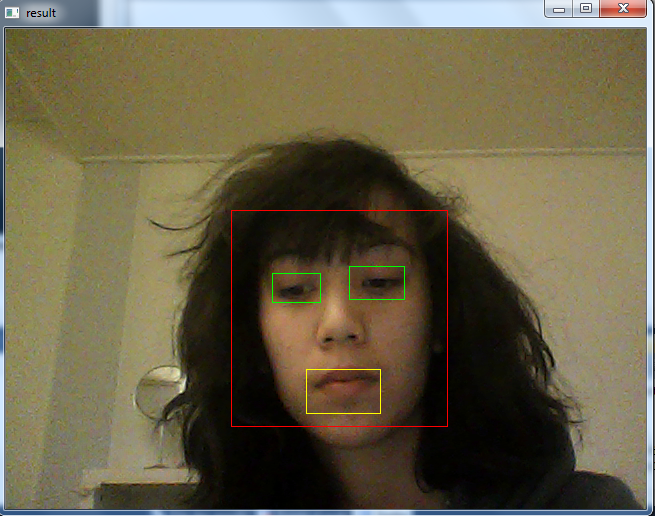
\includegraphics[scale=0.4]{figures/violajones_implementation_example} 
\newline
\caption{Example of face and ROI detection with Viola-Jones}
\label{violajones_implementation_example}
\end{center} 
\end{figure}
%\newpage
  \begin{titlepage}
    \vspace*{\fill}
      \part{Feature extraction}
    \vspace*{\fill}
  \end{titlepage}

\startcontents[parts]

\phantomsection
\chapter*{Contents}

\textit{This part will focus on the step following face detection, which is feature extraction. Chapter~\ref{chap:extraction} will present the main issues on feature extraction, and usual feature extraction methods, while the following chapter will focus on the Local Binary Patterns algorithm.} 

\vspace{\baselineskip}

\printcontents[parts]{}{-1}{\setcounter{tocdepth}{1}}

\pagebreak
\phantomsection
\chapter{Feature extraction}
\label{chap:extraction}

\noindent After having detected the face, for example using Viola-Jones algorithm, it is necessary to perform feature extraction in order to process data before classification. 
This step takes an image as input, and extracts vectors characterizing its main features. In the case of a facial expression recognition system, resulting vectors contain informations about spacial configuration of facial features, but can also encode informations about shape, texture or movement of the image's content \cite{CHI03}.
\newline

\noindent There are however many kinds of algorithms outputting features vectors, and the choice of an effective one depends on many criteria. These feature extration methods can generally be ranked among 2 categories: they can either be appearance-based or geometry-based, depending on the way they extract feature vectors. The aim of this chapter is to explain the differences between these 2 types of feature extraction methods, and provide some examples from each category.
\newline

\vspace{\baselineskip}
\noindent Before developing a facial expression recognition project, it is important to know what already exists; the state of the art of facial expression recognition system. In this chapter, an overview will be given of the existing systems before to decide on a feature extraction system for the project.
\newline

\noindent Two main categories of feature extraction algorithms can be distinguished : \textit{appearance-based} or \textit{geometry-based}. The first ones are algorithms that try to find basic vectors characterizing the whole picture, usually by a dimensionality reduction method. These algorithms lead to a simplification of the dataset, while retaining the main characteristics of the picture. However, these methods have to be carefully parametrized, so they do not encounter the "curse of dimensionality", which is about processing high-dimensional data.
\vspace{\baselineskip}

\noindent Examples of appearance-based methods : Principal Component Analysis, Linear Discriminant Analysis, Hidden Markov Models, Eigenfaces.
\newline

\noindent The second type of feature extraction algorithms are geometry-based algorithms. These methods tend to locate important features, and build the feature vectors depending on those regions of interest. The key point of these methods is that the face is not a global structure anymore. Indeed, it has been summarized in a set of features regions, which are themselves translated into feature vectors.
\vspace{\baselineskip}

\noindent Examples of geometry-based methods : Gabor Wavelets, Local Binary Patterns.
\newline

\section{Principal Component Analysis (PCA)}

\vspace{\baselineskip}
\noindent This is a statistical method; one of the most used in linear algebra. PCA is mainly used to reduce high dimensionality of data and to obtain the most important information out of it. PCA computes a covariance matrix and a set of values called the eigenvalues and eigenvectors from the original data \cite{GAN08}. Its output is a new coordinate system with lower dimensions, obtained from transformed high dimensionality of data, while preserving the most important information.  Since it is a statistical method, it can also be used in the classification step.
\newline

\section{Linear Discriminant Analysis (LDA)}

\vspace{\baselineskip}
\noindent Linear Discriminant Analysis is also a statistical method, used to classify a set of objects into groups. It is done by looking at a specific set of features describing the objects. LDA as PCA are used to establish a linear relationship between the dimensions of the data. LDA uses this relationship to model the differences into classes, while PCA does not take any differences into account in the linear relationship. The idea behind LDA  is to perform a linear transformation on the data to obtain a lower dimensional set of features \cite{GAN08}. Like PCA, LDA can also be used as a classification algorithm.
\newline

\section{Local Binary Patterns (LBP)}

\vspace{\baselineskip}
\noindent This is an geometry-based method. Its first application was to describe texture and shape of an image by extracting informations from the neighbourhood of a central pixel. These informations are the output of the thresholding of intensity values from the neighbourhood pixels with the intensity value of the central pixel \cite{GAN08}. This method will be detailed in Chapter \ref{chap:lbp}, and will be used in our facial expression recognition system.
\newline

\section{Hidden Markov Models (HMM)}

\vspace{\baselineskip}
\noindent These models are a set of statistical models used to characterize the statistical properties of a signal \cite{RAB93}. It can be used as a classification algorithm, and can also be developed to recognize expressions based on the "maximum likelihood decision criterion" \cite{LIE98}.
\newline

\section{Eigenfaces}

\vspace{\baselineskip}
\noindent Eigenfaces are a set of eigenvectors. These eigenvectors are derived from the covariance matrix of a set of images; and this in a high-dimensional vector space. The eigenvectors are ordered and each one represents the different amount of the variation among images. Characterization of the variation between face images is then possible \cite{TUR91}.
\newline

\section{Gabor Filters}

\vspace{\baselineskip}
\noindent Gabor filters are applied in order to extract a set of Gabor wavelet coefficients. Filter responses are obtained when Gabor filters are convolved with face image. These representations of face image display desirable locality and orientation performance \cite{JEM09}. However, the main limitation of the Gabor feature extraction is processing time.This algoritm is very time-consuming, and dimensions of resulting vectors are prohibitively large \cite{PRA09}.
\newline

\noindent Conclusion paragraph that opens on LBP


\newpage
\phantomsection
\chapter{Local Binary Patterns}
\label{chap:lbp}

\noindent bla

\section{Overview}

\noindent bla
\newline

\section{Histogram computing}

\noindent bla
\newline

\section{Improvements}

\noindent bla
\newline

\subsection{Circular LBP}

\vspace{\baselineskip}
\noindent bla
\newline

\subsection{Uniform LBP}

\vspace{\baselineskip}
\noindent bla
\newline

\stopcontents[parts]



%\newpage
  \begin{titlepage}
    \vspace*{\fill}
      \part{Feature extraction and classification}
    \vspace*{\fill}
  \end{titlepage}

\startcontents[parts]

%\chapter{Introduction}\label{ch:introduction}
\phantomsection
\chapter*{Contents}

\textit{This part will focus on the steps following face detection, which are feature extraction and classification. Chapter~\ref{chap:extraction} will present the main issues on feature extraction, and usual feature extraction methods, while the next chapter will focus on the Local Binary Patterns algorithm. Classification will then be introduced in Chapter~\ref{chap:classification}, with a general overview of the classification problem, along with a presentation of some classification algorithms. The last chapter will describe Support Vector Machine classification.}

\vspace{\baselineskip}

\printcontents[parts]{}{-1}{\setcounter{tocdepth}{1}}

\pagebreak

\phantomsection
\chapter{Feature extraction}
\label{chap:extraction}

\noindent After having detected the face, for example using Viola-Jones algorithm, it is necessary to perform feature extraction in order to process data before classification. 
This step takes an image as input, and extracts vectors characterizing its main features. In the case of a facial expression recognition system, resulting vectors contain informations about spacial configuration of facial features, but can also encode informations about shape, texture or movement of the image's content \cite{CHI03}.
\newline

\noindent There are however many kinds of algorithms outputting features vectors, and the choice of an effective one depends on many criteria. These feature extration methods can generally be ranked among 2 categories: they can either be appearance-based or geometry-based, depending on the way they extract feature vectors. The aim of this chapter is to explain the differences between these 2 types of feature extraction methods, and provide some examples from each category.
\newline

\vspace{\baselineskip}
\noindent Before developing a facial expression recognition project, it is important to know what already exists; the state of the art of facial expression recognition system. In this chapter, an overview will be given of the existing systems before to decide on a feature extraction system for the project.
\newline

\noindent Two main categories of feature extraction algorithms can be distinguished : \textit{appearance-based} or \textit{geometry-based}. The first ones are algorithms that try to find basic vectors characterizing the whole picture, usually by a dimensionality reduction method. These algorithms lead to a simplification of the dataset, while retaining the main characteristics of the picture. However, these methods have to be carefully parametrized, so they do not encounter the "curse of dimensionality", which is about processing high-dimensional data.
\vspace{\baselineskip}

\noindent Examples of appearance-based methods : Principal Component Analysis, Linear Discriminant Analysis, Hidden Markov Models, Eigenfaces.
\newline

\noindent The second type of feature extraction algorithms are geometry-based algorithms. These methods tend to locate important features, and build the feature vectors depending on those regions of interest. The key point of these methods is that the face is not a global structure anymore. Indeed, it has been summarized in a set of features regions, which are themselves translated into feature vectors.
\vspace{\baselineskip}

\noindent Examples of geometry-based methods : Gabor Wavelets, Local Binary Patterns.
\newline

\section{Principal Component Analysis (PCA)}

\vspace{\baselineskip}
\noindent This is a statistical method; one of the most used in linear algebra. PCA is mainly used to reduce high dimensionality of data and to obtain the most important information out of it. PCA computes a covariance matrix and a set of values called the eigenvalues and eigenvectors from the original data \cite{GAN08}. Its output is a new coordinate system with lower dimensions, obtained from transformed high dimensionality of data, while preserving the most important information.  Since it is a statistical method, it can also be used in the classification step.
\newline

\section{Linear Discriminant Analysis (LDA)}

\vspace{\baselineskip}
\noindent Linear Discriminant Analysis is also a statistical method, used to classify a set of objects into groups. It is done by looking at a specific set of features describing the objects. LDA as PCA are used to establish a linear relationship between the dimensions of the data. LDA uses this relationship to model the differences into classes, while PCA does not take any differences into account in the linear relationship. The idea behind LDA  is to perform a linear transformation on the data to obtain a lower dimensional set of features \cite{GAN08}. Like PCA, LDA can also be used as a classification algorithm.
\newline

\section{Local Binary Patterns (LBP)}

\vspace{\baselineskip}
\noindent This is an geometry-based method. Its first application was to describe texture and shape of an image by extracting informations from the neighbourhood of a central pixel. These informations are the output of the thresholding of intensity values from the neighbourhood pixels with the intensity value of the central pixel \cite{GAN08}. This method will be detailed in Chapter \ref{chap:lbp}, and will be used in our facial expression recognition system.
\newline

\section{Hidden Markov Models (HMM)}

\vspace{\baselineskip}
\noindent These models are a set of statistical models used to characterize the statistical properties of a signal \cite{RAB93}. It can be used as a classification algorithm, and can also be developed to recognize expressions based on the "maximum likelihood decision criterion" \cite{LIE98}.
\newline

\section{Eigenfaces}

\vspace{\baselineskip}
\noindent Eigenfaces are a set of eigenvectors. These eigenvectors are derived from the covariance matrix of a set of images; and this in a high-dimensional vector space. The eigenvectors are ordered and each one represents the different amount of the variation among images. Characterization of the variation between face images is then possible \cite{TUR91}.
\newline

\section{Gabor Filters}

\vspace{\baselineskip}
\noindent Gabor filters are applied in order to extract a set of Gabor wavelet coefficients. Filter responses are obtained when Gabor filters are convolved with face image. These representations of face image display desirable locality and orientation performance \cite{JEM09}. However, the main limitation of the Gabor feature extraction is processing time.This algoritm is very time-consuming, and dimensions of resulting vectors are prohibitively large \cite{PRA09}.
\newline

\noindent Conclusion paragraph that opens on LBP


\newpage
\phantomsection
\chapter{Local Binary Patterns}
\label{chap:lbp}

\noindent bla

\section{Overview}

\noindent bla
\newline

\section{Histogram computing}

\noindent bla
\newline

\section{Improvements}

\noindent bla
\newline

\subsection{Circular LBP}

\vspace{\baselineskip}
\noindent bla
\newline

\subsection{Uniform LBP}

\vspace{\baselineskip}
\noindent bla
\newline
\pagebreak
\newpage
\phantomsection
\chapter{Classification}
\label{chap:classification}

\noindent Classification is done through machine learning algorithms. Machine learning, being a branch of Artificial Intelligence, aims to helps AI systems improve their performances by learning from their environment. Indeed, the knowledge necessary to build a robust and intelligent system can not always be built-in or explained to it. The solution to this problem is to make the system learn this knowledge through examples and apply it to similar situations. Thus it will be able to perform relevant actions without the need of human intervention. 
\newline

\noindent More specifically, machine learning can be described as a way to develop and implement algorithms taking empirical data as input, and processing these values in order to find links between them. The output will then be used by the system to compute the appropriate action or behaviour. In order to achieve that, the system needs to learn key characteristics from a training dataset given as example or obtained through past experience. It will then study this observable data, and build a model based on it. The system will then use this model to infer actions depending on new data it will get as input.
\newline

\noindent However, machine learning is not only about computing a database and relying on it for every possible situation. In a changing environment, the system needs to know how to learn from these changes and adapt itself.
\newline

\noindent There are many kinds of machine learning algorithms, with their own specificities and level of abstraction. In this chapter we will focus on algorithms behaving like functions and performing pattern recognition. Indeed, a facial image is a set of patterns of different sizes and shapes. Pattern recognition through machine learning can be divided into two main categories of algorithms: supervised learning and unsupervised learning. Those two categories will be described further in this chapter, along with examples.
\newline

\noindent This chapter serves as an introduction for Chapter \ref{chap:svm}, which is about Support Vector Machines, a specific kind of supervised learning algorithm which will be used in our system.
\newline

\phantomsection
\section{Supervised learning}

\vspace{\baselineskip}
\noindent Supervised learning is the task of providing labelled input data to the algorithm, also called \textit{train data}. The main point is that the model is only defined by the observable data it gets for training. It does not make any assumption about underlying, latent variables that could interfere with this observable data. It can then search for patterns and relations between the data points, and build a model fitting these relations before classifying test data.
\newline

\noindent Classification can be divided in two steps, first step being training, and second step being prediction. There are many kinds of supervised learning algorithms, the basic one being a naive Bayes classifier, which will be detailed afterwards. An other example of algorithm is linear discriminant analysis (LDA). Furthermore, the next chapter will focus on an other supervised learning algorithm: Support Vector Machine.
\newline

\subsection{Naive Bayes classifier}

\vspace{\baselineskip}
\noindent The Bayesian classifier is based on Bayes theorem:
\newline

\begin{equation}
    \begin{array}{ll}
        \text{\textbf{sum rule: }} & p(X) = \sum\limits_{Y} p(X,Y) \\
        \text{\textbf{product rule:}} & p(X,Y) = p(Y|X)p(X)
    \end{array}
    \label{bayes}
\end{equation}

\vspace{\baselineskip}
\noindent With these rules, it is possible to compute the \textit{posterior probability} of an event $C_i$ given observable data $x$, using formula \ref{posterior}.

\begin{equation}
	p(C_i|x) = \frac{p(x|C_i \times p(C_i)}{p(x)}
	\label{posterior}
\end{equation}

\noindent With:
\begin{itemize}
\item $p(x|C_i)$ the probability of observed data $x$ given $C_i$, which can also be called the \textit{likelihood function of $C_i$};
\item $p(C_i)$ the prior probability of $C_i$;
\item $p(x)$ the probability of observable data $x$.
\end{itemize} 

\noindent When combined with Bayes theorem, equation \ref{posterior} becomes:

\begin{equation}
	p(C_i|x) = \frac{p(x|C_i \times p(C_i)}{\sum\limits_{k=1}\limits^{K} p(C_k) \times p(x|C_k)}
	\label{posterior_bayes}
\end{equation}

\noindent The classifier output will then be class $C_i$ which meets condition $p(C_i|x) = \max \limits_{k} p(C_k|x)$ (the likelihood function has to be the highest among all classes $C_k$).

\subsection{Linear Discrimination}

\vspace{\baselineskip}
\noindent Since classification is the process of assigning the input vector $x$ to one of the classes $C_i$, $i=1, ..., I$, its key point is about learning the decision boundaries that separate the different classes in the input space \cite{BIS06}. If the input dataset is \textit{linearly separable}, decision boundaries can then be described by linear functions of the input vector $x$.
\newline

\noindent For example, the linear discriminant function for a 2-class problem will look like 

\begin{equation}
y(x) = w^Tx + \omega_0
\end{equation}

\noindent With \textit{weight vector} $w^T$ and \textit{bias} $\omega_0$ \cite{BIS06}. The input vector $x$ is then assigned to class $C_1$ if $y(x) = 0$, otherwise it will be classified as belonging to class $C_2$.
\newline

\noindent For problems with a number of classes K > 2, a \textit{one-versus-the-rest} approach can be used, where K-1 two-way discriminant functions are used: the $k^{th}$ discriminant function will determine if a point belongs to class $C_k$ or not. However, as shown in Figure \ref{one_vs_rest}, this combination of discriminant functions leaves an ambiguous region \cite{BIS06}. 
\newline

\begin{figure}[!h]
\begin{center}
\noindent 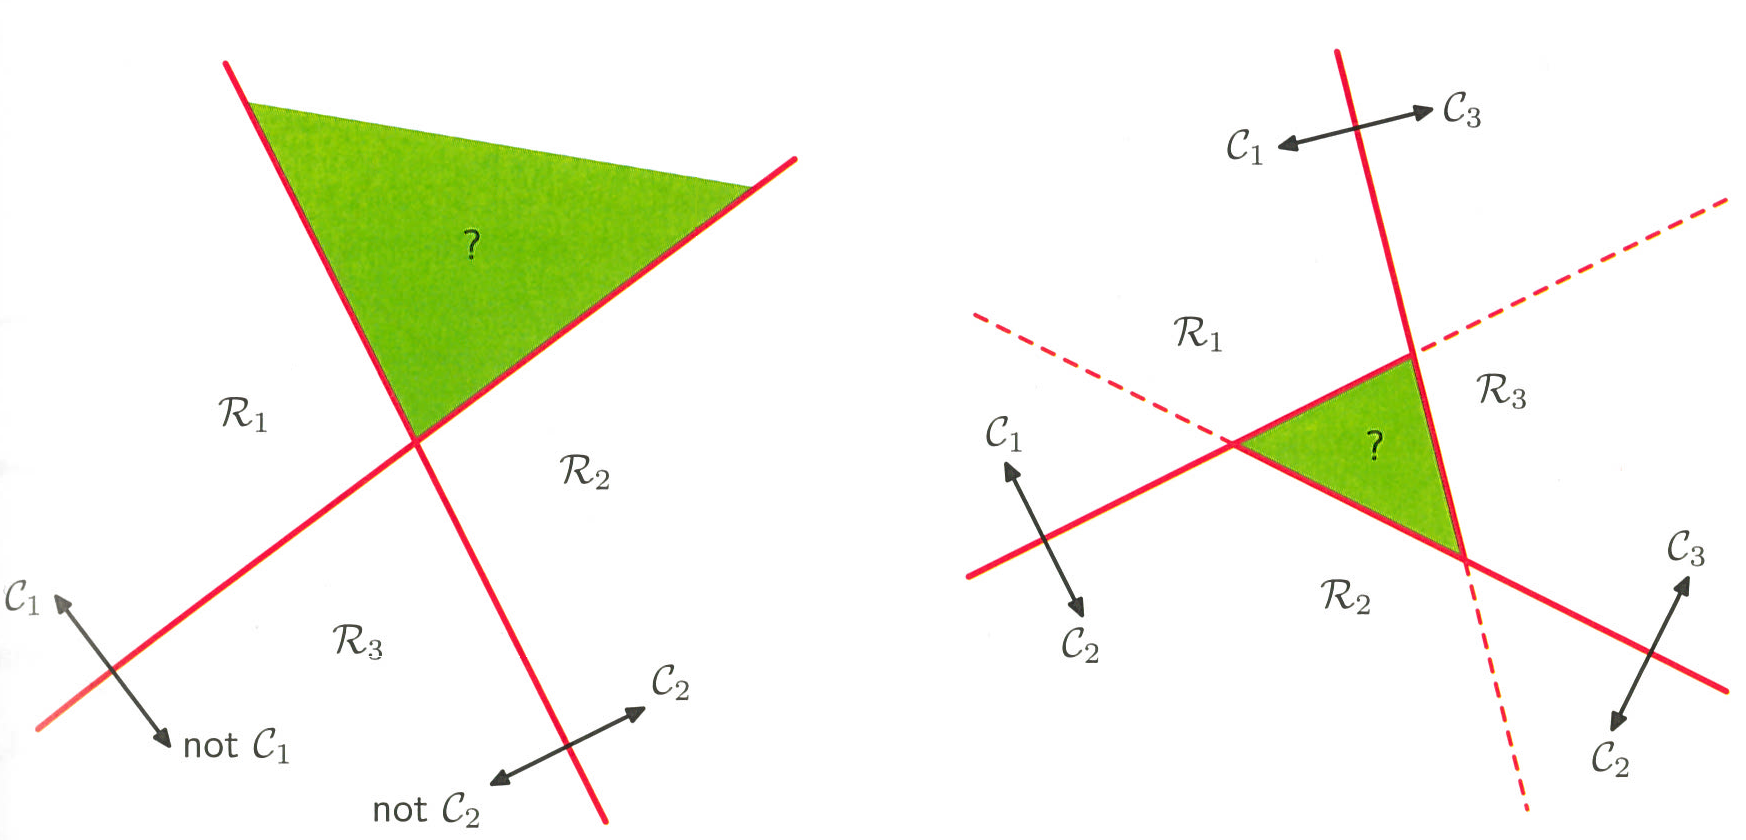
\includegraphics[scale=0.2]{figures/one_vs} 
\newline
\caption{Attempting to construct a $K$ class discriminant from a set of two class discriminants leads to ambiguous regions, shown in green. On the left is an example of \textit{one-versus-the-rest} approach, the discriminant function designed to separate points belonging to a class $C_i$ and points that are not. On the right is an example of \textit{one-versus-all} approach involving 3 discriminant functions, each one separating a pair of classes classes $C_i$ and $C_j$.From: Christopher M. Bishop, \textit{Pattern Recognition and Machine Learning}. Copyright \copyright  2006 by Springer Science.}
\label{one_vs_rest}
\end{center} 
\end{figure}

\noindent An other way to solve a multi-class problem could be to use $\frac{K(K-1)}{2}$ discriminant functions, which is the \textit{one-versus-all} approach. However, the resulting K-class discriminant also has an ambiguous region problem, as seen in Figure \ref{one_vs} \cite{BIS06}.
\newline

\noindent A K-class discriminant which does not lead to an ambiguous region problem is to use K linear discriminant functions $g(x)_k$, $k=1..K$, and to assign an input vector $x$ to a class $C_i$ if $g(x)_i = \max\limits_{k} g_k(x)$. Indeed, as shown in Figure \ref{k_discr}, there are no more ambiguous regions \cite{BIS06}.
\newline

\begin{figure}[!h]
\begin{center}
\noindent 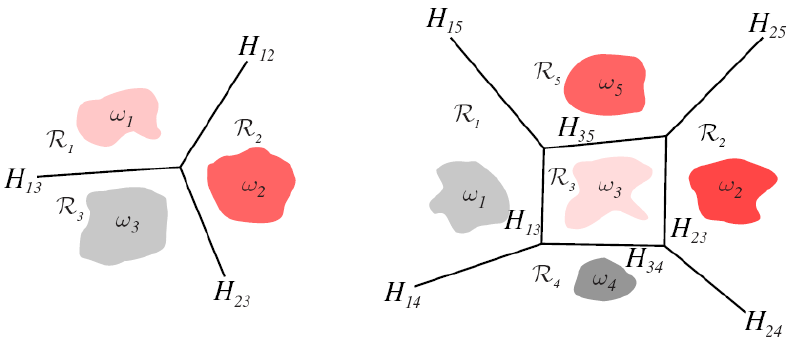
\includegraphics[scale=0.5]{figures/lda_k_disc} 
\newline
\caption{Decision boundaries produced by a linear machine for a 3-class problem and a 5-class problem. From: Richard O. Duda, Peter E. Hart, and David G. Stork, \textit{Pattern Classification}. Copyright \copyright  2001 by John Wiley \& Sons Inc.}
\label{k_disc}
\end{center} 
\end{figure}

\phantomsection
\section{Unsupervised learning}

\vspace{\baselineskip}
\noindent Unlike supervised learning, the classification algorithm is not fed with train data in the case of unsupervised learning. It will be given a set of observable data, and its goal is to group data the smartest way possible, and by itself. Furthermore, in unsupervised learning, the concept of \textit{class} is not applicable any more; the term \textit{cluster} being preferred.
\newline

\noindent The key point of unsupervised algorithms is data clustering. In most common unsupervised algorithms such as K-means, the algorithm can get a hint of the number of clusters it has to find. It then proceeds, usually in an iterative way, to find the latent variables related to the data. Indeed, it is assumed that all observable data is governed by latent variables which can be organized in different levels.
\newline

\noindent Besides K-means, an other common unsupervised algorithm is the Mixture Models algorithm, which will also be described in the following subsections.
\newline

\subsection{K-Means}

\vspace{\baselineskip}
\noindent K-means clustering relies on a set of k reference vectors $\mu_k$, $k=1..K$, also called \textit{prototype vectors}. These vectors represent the centres of the K clusters. This clustering method has two goals: first, it has to find how the clusters are shaped and which data lies in which cluster; secondly, the set of vectors $\{\mu_k\}$ has to be determined while verifying the following condition: for each data point $x_n$, the sum of squares of the distances between $x_n$ and its closest vector $\mu_k$ is a minimum. In other words, equation \ref{distort_fc}, also called \textit{distortion function} has to be minimized \cite{BIS06}.

\begin{equation}
J = \sum\limits_{n=1}\limits^{N} \sum\limits_{k=1}\limits^{K} r_{nk} ||x_n - \mu_k||^2
\label{distort_fc}
\end{equation}

\noindent With

\begin{equation*}
r_{nk} = \left\{
	\begin{array}{ll}
		1 & \mbox{if }  k = arg \min_j ||x_n - \mu_j||^2 \\
		0 & \mbox{otherwise}
	\end{array}
\right.
\end{equation*}
\vspace{\baselineskip}

\noindent This can be achieved through the following iterative algorithm, which result can be seen in Figure \ref{k-mean_res}:
\newline

\begin{algorithmic}
\State Initialization of reference vectors $\mu_k$, $k = 1..K$ 
\Repeat	
	\ForAll{$x_n \in \chi$}
		\State \begin{math} 
			r_{nk} \gets \left\{
			\begin{array}{ll}
				1 & \mbox{if }  k = arg \min_j ||x_n - \mu_j||^2 \\
				0 & \mbox{otherwise}
			\end{array}
			\right.
			\end{math}
	\EndFor
	\ForAll{$\mu_k$, $k = 1..K$ }
		\State $\mu_k \gets \frac{\sum\limits_n r_{nk}x_n}{\sum\limits_n r_{nk}}$
	\EndFor
\Until{$\mu_k$ converge}
\end{algorithmic}

\vspace{\baselineskip}

\begin{figure}[!h]
\begin{center}
\noindent 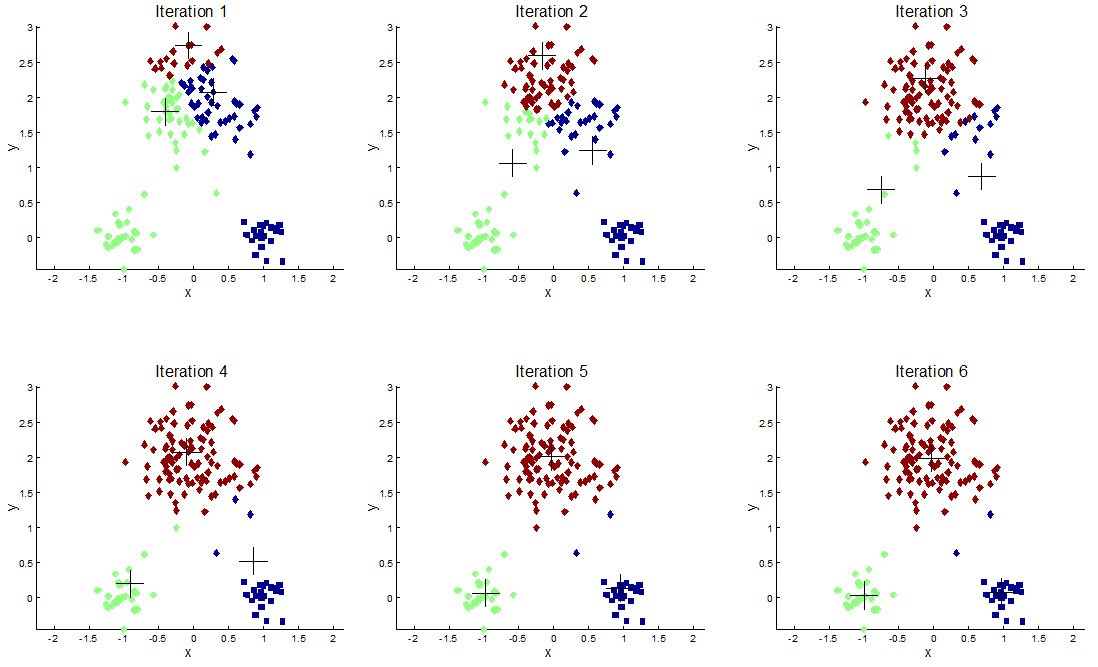
\includegraphics[scale=0.5]{figures/k-mean_res} 
\newline
\caption{Example of application of the iterative K-means algorithm.}
\label{k-mean_res}
\end{center} 
\end{figure}

\noindent In this algorithm, denominator $\sum\limits_n r_{nk}$ corresponds to the number of points assigned to cluster $k$, which sets $\mu_k$ as the mean of the cluster, hence the name \textit{K-means algorithm} \cite{BIS06}.
\newline

\noindent This algorithm can also be used in \textit{lossy data compression}, where input data can be reconstructed with minor errors, in contrary to \textit{lossless data compression}. If the K-means algorithm is applied, then for each data point $x_n$ the only value stored is the cluster $k$ it belongs to. Apart from the data points, values of cluster centres $\mu_k$ are also stored. Hence, during data reconstruction, each data point is approximated by corresponding vector $\mu_k$. This approximation is called \textit{vector quantization} \cite{BIS06}.
\newline

\subsection{Mixture of Gaussians}

\vspace{\baselineskip}
\noindent While the K-means algorithm will try to find reference vectors describing the different clusters, the mixture models algorithm will rather model the underlying distribution of the clusters, usually by a Gaussian probability density function. Each cluster is then represented by a Gaussian distribution, and the aim of the algorithm is to find the best parameters for the latent variables governing these distributions. It can be achieved by finding parameters maximizing likelihood $p(x)=p(x|G_i)p(G_i)$, with:

\begin{itemize}
\item $G_i$: clusters
\item $p(G_i)$: prior probability (mixture proportion)
\item $p(x|G_i)$: component density
\end{itemize}

\noindent Since a Gaussian mixture is roughly similar to $p(x|G_i) \sim \mathcal{N}(\mu_i, \Sigma_i)$, with mean vector $\mu_i$ and covariance matrix $\Sigma_i$, the goal is now to maximize the log likelihood function described in Equation \ref{log_likelihood}.

\begin{equation}
\begin{array}{ll}
\mathcal{L}(\Phi|\chi) & = \ln \prod\limits_n p(x^n | \Phi) \\
 & = \sum\limits_{n=1}\limits^{N} \left\{ \sum \limits_{k=1}\limits^{K} \pi_k \mathcal{N}(x_n|\mu_k, \Sigma_k)\right\}
\end{array}
\label{log_likelihood}
\end{equation}

\noindent with $\Phi$ representing mixing coefficients, including prior probabilities and sufficient statistics of component densities.
\newline

\noindent The maximum likelihood estimation can then be obtained through the \textit{Expectation-Maximization algorithm} for Gaussian Mixture Models (EM), which converges into a result comparable as the one in Figure \ref{mixture_model} \cite{BIS06}.
\newline

\noindent \textbf{Expectation-Maximization algorithm:}
\newline

\begin{algorithmic}
\State Initialize means $\mu_n$, covariances $\Sigma_n$, mixing coefficients $\pi_n$ and compute initial value of the log likelihood

\Repeat
	\State \textbf{Expectation step}: Evaluate the expected value of the latent variable using current parameter values:
		\State $\gamma(z_{nk}) = 
		\frac{\pi_k\mathcal{N}(x_n|\mu_k, \Sigma_k)}{\sum\limits_{j=1}\limits^{K}\pi_j\mathcal{N}(x_n|\mu_j, \Sigma_j)}$
	\State \textbf{Maximization step}: Re-estimate the parameters using $\gamma(z_{nk})$:
		\State $\pi^{new}_k = \frac{N_k}{N}$
		\State $\mu^{new}_k = \frac{1}{N_k}\sum\limits_{n=1}\limits{N}\gamma(z_{nk})x_n$
		\State $\Sigma^{new}_k = \frac{1}{N_k}\sum\limits_{n=1}\limits{N}\gamma(z_{nk}) (x_n - \mu^{new}_k) (x_n - \mu^{new}_k)^T$
		\State Where $N_k = \sum\limits_{n=1}\limits{N}\gamma(z_{nk})$
	\State Evaluate log likelihood $\mathcal{L}$ 
\Until {$\mathcal{L}$ converges}
\end{algorithmic}

\begin{figure}[!h]
\begin{center}
\noindent 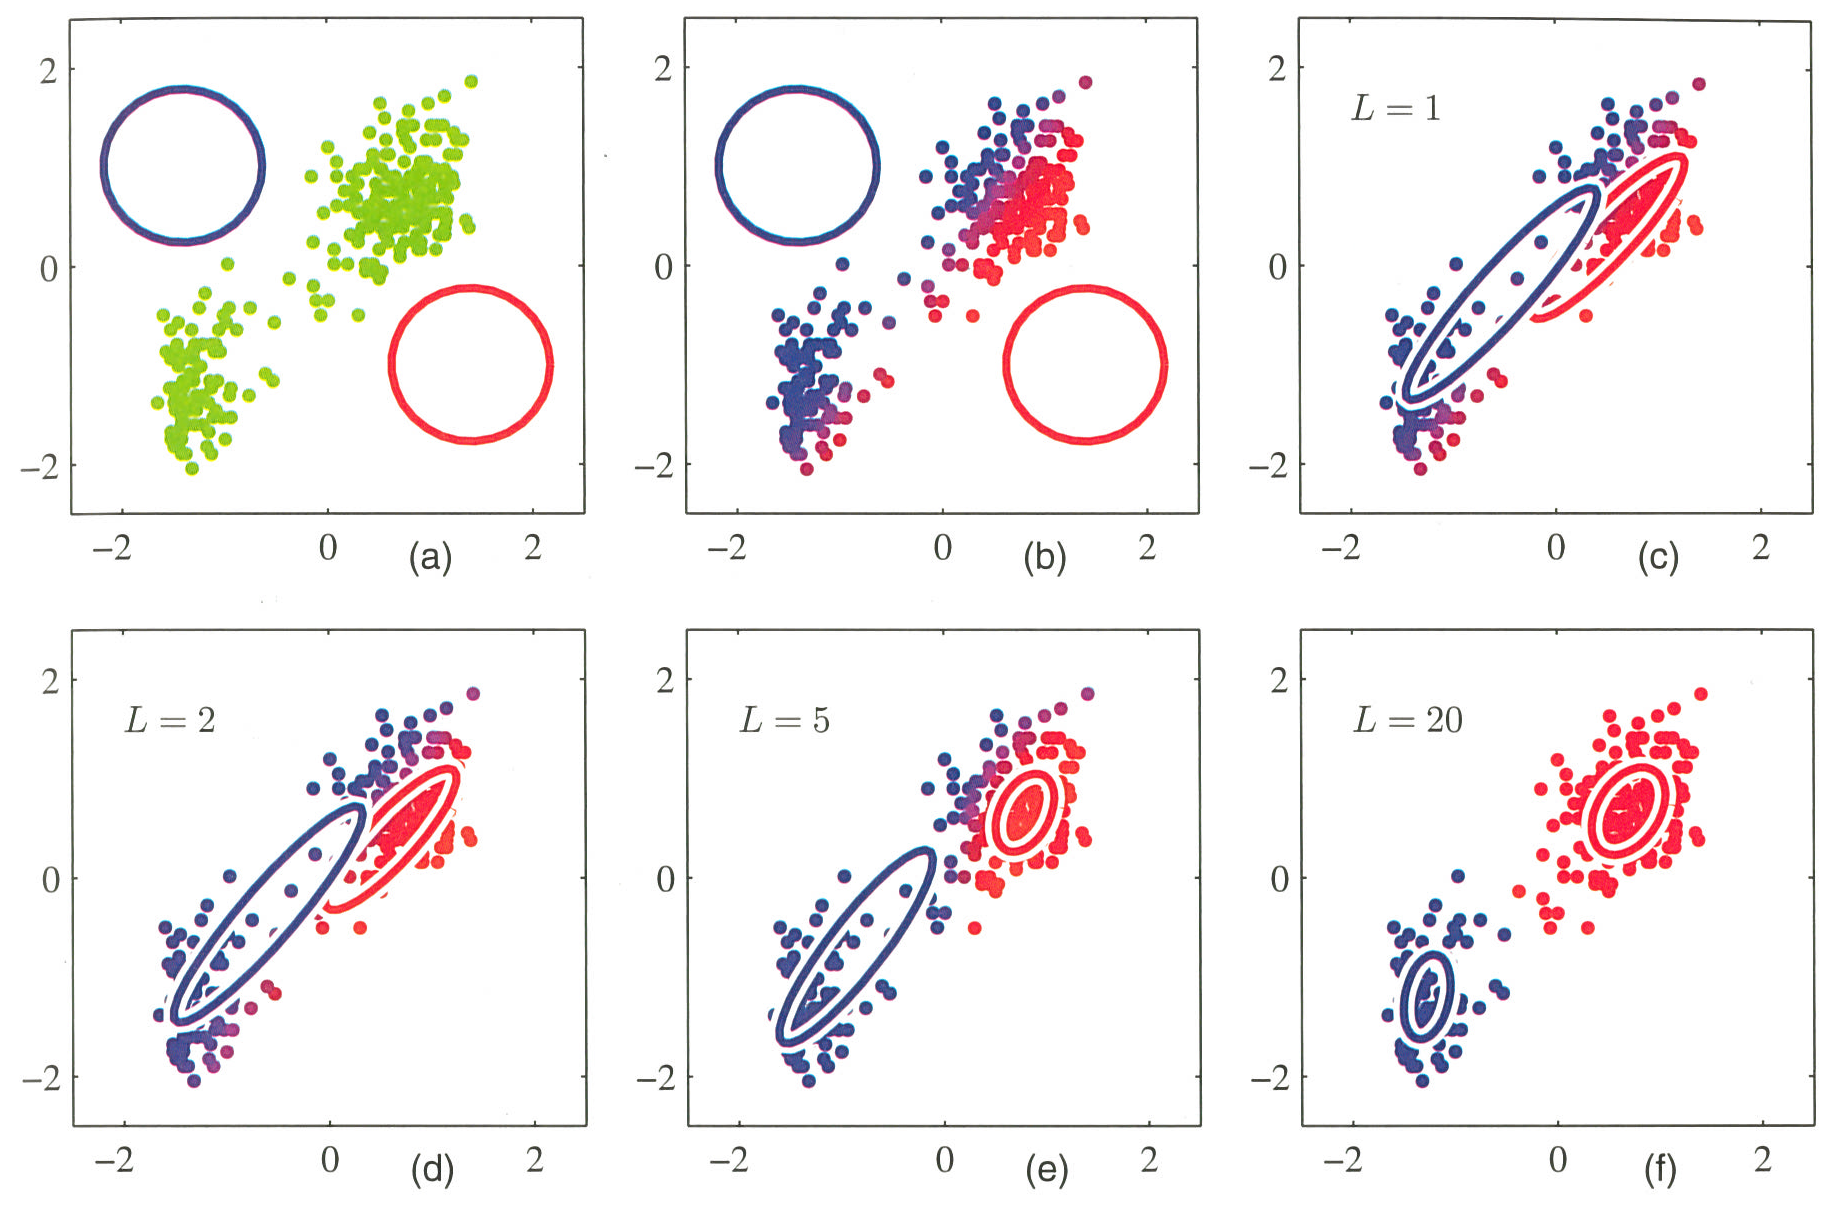
\includegraphics[scale=0.2]{figures/mixture_model} 
\newline
\caption{Illustration of the EM algorithm. From: Christopher M. Bishop, \textit{Pattern Recognition and Machine Learning}. Copyright \copyright  2006 by Springer Science.}
\label{mixture_model}
\end{center} 
\end{figure}
\pagebreak

\newpage
\phantomsection
\chapter{Support Vector Machine}
\label{chap:svm}

\noindent Support Vector Machine (SVM) is a binary linear classifier belonging to the supervised learning algorithms category. It has been proven to be very efficient for classification, regression and novelty detection problems \cite{BIS06}, which makes it suitable for facial expression recognition.
\newline

\noindent This chapter will first provide an overview of how classification is performed using SVM. It will then focus and describe the key points behind this classifier, namely \textit{margin maximization} and \textit{kernel function}. The chapter will conclude with the review of a research paper detailing facial expression recognition using LBP for feature extraction and SVM for classification.
\newline

\phantomsection
\section{Overview}
\label{svm_overview}

\vspace{\baselineskip}
\noindent SVM is originally a binary classifier, which means it has a \textit{one-vs-all} approach. It is a decision machine, so its output is not a posterior probability, but rather a class label \cite{BIS06}.  It can be adapted into a \textit{relevance vector machine} to output posterior probabilities though \cite{BIS06}, but this alternative will not be detailed in our report.
\newline

\noindent SVM is also a linear classifier, such as LDA. For a two-class problem, it will linearly separate the train data by finding the optimal hyperplane between these 2 classes. This hyperplane is defined as being as far as possible from both classes. \textit{Margin maximization} is then applied to optimize the distance between the two classes and the hyperplane, as it will be explained in Section \ref{margin_max}.
\newline

\noindent The name "Support Vector" originates from the margin maximization feature. Indeed, the distance between the classes and the separating hyperplane is computed regarding to the closest data points from both classes. These particular data points, lying on the margins edges, are the support vectors. Some properties are associated to these vectors, such as non-zero Lagrange multipliers (see Section \ref{margin_max}), which builds the classification algorithm.
\newline

\noindent For a multi-class problem, however, this linear separation is not possible anymore. The dataset has to be mapped into an other space, where it can be linearly separated. This is what \textit{kernel functions} are used for, as described in Section \ref{kernel_fct}.
\newline

\phantomsection
\section{Margin maximization}
\label{margin_max}

\vspace{\baselineskip}
\noindent As introduced in Section \ref{svm_overview}, margin maximization for a two-class linear problem starts by finding the separating hyperplane between these two classes. A linear classification model of the form $f(x) = w(x) + b$ can be inferred, with $w$ being the normal to the hyperplane and $b$ the bias. The hyperplane can then be characterized by  $w(x) + b = 0$.
\newline

\noindent Margin is defined as the distance between the closest point of the class to the hyperplane, and that hyperplane, which can also be written as $ d(x) = \frac{|w(x) + b |}{||w||}$. Since a data point $(x_i, y_i)$ is correctly classified if $yf(x) \geq 1$, maximizing the margin is the action of maximizing $||w||^{-1}$, which is consequently equivalent to minimizing $||w||^2$ depending on this constraint. Margin maximization then requires to solve a \textit{quadratic programming} problem under constraints, as seen in Equation \ref{margin_max_eq}.

\begin{equation}
\left\{
\begin{array}{l}
\min \frac{1}{2} ||w||^2 \\
\forall i, \, y_i . f(x) \geq 1
\end{array}
\right.
\label{margin_max_eq}
\end{equation}

\vspace{\baselineskip}

\phantomsection
\section{Kernel function}
\label{kernel_fct}

\vspace{\baselineskip}
\noindent It might however not be possible to perform this linear separation with more classes. Indeed, data might be overlapping, and thus it will not be a linear problem anymore. The solution to overcome this problem is to map the non-linear dataset from its input space into a higher feature space using a function $\Phi(x)$, and perform margin maximization and classification in this higher space. 
\newline

\noindent In order to achieve this mapping, a \textit{kernel function} of the form $K(x_i, x_j) = \Phi(x_i)^T \Phi(x_j)$ is applied to the dataset. This kernel represents an inner product in the feature space. There are four kernels available, which are described in Equation \ref{kernels_svm}.
\newline

\begin{equation}
\begin{array}{ll}
	\text{Linear kernel:} & K(x_i,x_j) = x_i^Tx \\
	\text{Polynomial kernel:} & K(x_i,x_j) = (\gamma x_i^Tx_j + r)^T, \gamma > 0 \\
	\text{Radial Basis Function (Gaussian) kernel:} & K(x_i,x_j) = \exp(-\gamma \| x_i - x_j \|^2), \gamma > 0 \\
	\text{Sigmoid kernel:} & K(x_i,x_j) = \tanh(\gamma x_i^T x_j + r)\\
\end{array}
\label{kernels_svm}
\end{equation}

\noindent The main advantage of using a kernel function is that there is no need to define or calculate $\Phi(x_i)$, only $\Phi(x_i)^T \Phi(x_j)$. We hence do not know the true form of $\Phi(x_i)$. However, simple kernels are usually combined in order to build more complex ones.
\newline

\phantomsection
\section{Combining LBP and SVM}

\vspace{\baselineskip}
\noindent In a 2009 article, Shang and al \cite{SHA09} have performed facial expression recognition while using Local Binary Patterns for feature extraction, and comparing the accuracy of different kinds of classifiers:  template matching,  LDA and SVM. They have used images from the Cohn-Kanade database as train data, and the conclusion of their study is that classification using SVM has a high accuracy rate, as seen in Table \ref{accuracy_svm_lbp}. 
\newline

\begin{table}[h]
   \caption{\label{accuracy_svm_lbp} Recognition performance of LBP-based SVM with different kernels}
\begin{tabular}{|lcc|}
\hline
 & 6-Class recognition (\%) &  7-Class recognition (\%) \\
 \hline
 SVM (linear) & 91.5 $\pm$ 3.1 & 88.1 $\pm$ 3.8 \\
 SVM (polynomial) & 91.5 $\pm$ 3.1 & 88.1 $\pm$ 3.8 \\
 SVM (RBF) & 92.6 $\pm$ 3.1 & 88.9 $\pm$ 3.5 \\
 \hline
\end{tabular}
\end{table}

\noindent Furthermore, as seen in confusion matrices \ref{conf_mtx_6_svm_lbp} and \ref{conf_mtx_7_svm_lbp}, the accuracy for each facial expression is not the same. SVM has some difficulties especially when it comes to distinguish fear and sadness, the two facial expressions which have the lowest accuracy rates. Fear is mistaken with joy, while sadness is mistaken with anger or neutral state. Recognitions rates are however usually better for a 7-class classification, except for fear.
\newline

\noindent Since the accuracy of the system presented in this article is very high, we chose to implement a similar system. Indeed, we are performing facial expression recognition using LBP for feature extraction, and SVM classification. We however did not use the Cohn-Kanade database as train data. We will describe further our implementation and results further in the report. 
\newline

\begin{table}[h]
\caption{\label{conf_mtx_6_svm_lbp} Confusion matrix of 6-class facial expression recognition using SVM (RBF)}
\begin{tabular}{|lcccccc|}
\hline
 & Anger (\%) & Disgust (\%) & Fear (\%) & Joy (\%) & Sadness (\%) & Surprise (\%) \\
\hline
Anger & 89.7 & 2.7 & 0 & 0 & 7.6 & 0 \\
Disgust & 0 & 97.5 & 2.5 & 0 & 0 & 0 \\
Fear & 0 & 2.0 & 73.0 & 22.0 & 3.0 & 0 \\
Joy & 0 & 0.4 & 0.7 & 97.9 & 1.0 & 0 \\
Sadness & 10.3 & 0 & 0.8 & 0.8 & 83.5 & 4.6 \\
Surprise & 0 & 0 & 1.3 & 0 & 0 & 98.7 \\
\hline
\end{tabular}
\end{table}

\begin{table}[h]
\caption{\label{conf_mtx_7_svm_lbp} Confusion matrix of 7-class facial expression recognition using SVM (RBF)}
\begin{tabular}{|lccccccc|}
\hline
& Anger (\%) & Disgust (\%) & Fear (\%) & Joy (\%) & Sadness (\%) & Surprise (\%) & Neutral (\%) \\
\hline
Anger & 85.0 & 2.7 & 0 & 0 & 4.8 & 0 & 7.5 \\
Disgust & 0 & 97.5 & 2.5 & 0 & 0 & 0 & 0 \\
Fear & 0 & 2.0 & 68.0 & 22.0 & 1.0 & 0 & 7.0 \\
Joy & 0 & 0 & 0.7 & 94.7  & 1.1 & 0 & 3.5 \\
Sadness & 8.6 & 0 & 0 & 0 & 69.5 & 2.3 & 19.6 \\
Surprise & 0 & 0 & 1.3 & 0 & 0 & 98.2 & 0.5 \\
Neutral & 1.6 & 0.4 & 0 & 1.6 & 6.0 & 0.4 & 90.0 \\
\hline
\end{tabular}
\end{table}


\stopcontents[parts]



%\newpage
  \begin{titlepage}
    \vspace*{\fill}
      \part{Implementation}
    \vspace*{\fill}
  \end{titlepage}

\startcontents[parts]

\phantomsection
\chapter*{Contents}

\textit{In the previous parts, algorithms for feature detection and feature extraction were studied. A method for feature classification was also examined. This part will describe and explain how these algorithms and method are implemented.} 

\vspace{\baselineskip}

\printcontents[parts]{}{-1}{\setcounter{tocdepth}{1}}

\pagebreak
\phantomsection
\chapter{Face detection with Viola-Jones}
\label{chap:implementation_violajones}

\noindent The face detection part for this Facial Expression Recognition system is based on Viola-Jones face detection algorithm. This chapter describes how this Viola-Jones algorithm is used and implemented.
\newline

\phantomsection
\section{Viola-Jones}

\vspace{\baselineskip}
\noindent To perform Viola-Jones face detection, video sequences of face are obtained thanks to a webcam or to the Kinect. The algorithm is then able to detect face and regions of interest (ROI) in the frames. The regions of interest are the nose, the left eye, the right eye and the mouth. 
\newline

\noindent Classifiers are trained prior to be used. They are then loaded with a model; one for the face and one for each region of interest. Then, based on these classifiers, face and regions of interest are detected in the frames. Figure~\ref{violajones_implementation_example} shows an example of face detection,along with some regions of interest. In this case of ROI detection, different classifiers have been used for each eye. 
\newline

\begin{figure}[!h]
\begin{center}
\noindent 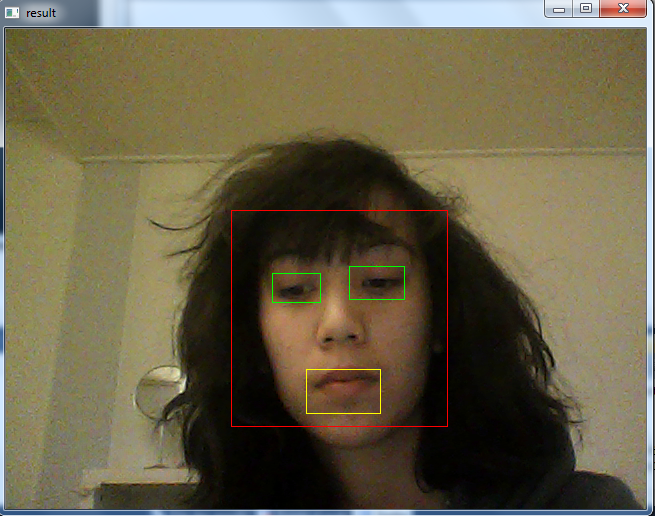
\includegraphics[scale=0.4]{figures/violajones_implementation_example} 
\newline
\caption{Example of face and ROI detection with Viola-Jones}
\label{violajones_implementation_example}
\end{center} 
\end{figure}
\clearpage
\newpage
%\newpage
  \begin{titlepage}
    \vspace*{\fill}
      \part{Feature extraction}
    \vspace*{\fill}
  \end{titlepage}

\startcontents[parts]

\phantomsection
\chapter*{Contents}

\textit{This part will focus on the step following face detection, which is feature extraction. Chapter~\ref{chap:extraction} will present the main issues on feature extraction, and usual feature extraction methods, while the following chapter will focus on the Local Binary Patterns algorithm.} 

\vspace{\baselineskip}

\printcontents[parts]{}{-1}{\setcounter{tocdepth}{1}}

\pagebreak
\phantomsection
\chapter{Feature extraction}
\label{chap:extraction}

\noindent After having detected the face, for example using Viola-Jones algorithm, it is necessary to perform feature extraction in order to process data before classification. 
This step takes an image as input, and extracts vectors characterizing its main features. In the case of a facial expression recognition system, resulting vectors contain informations about spacial configuration of facial features, but can also encode informations about shape, texture or movement of the image's content \cite{CHI03}.
\newline

\noindent There are however many kinds of algorithms outputting features vectors, and the choice of an effective one depends on many criteria. These feature extration methods can generally be ranked among 2 categories: they can either be appearance-based or geometry-based, depending on the way they extract feature vectors. The aim of this chapter is to explain the differences between these 2 types of feature extraction methods, and provide some examples from each category.
\newline

\vspace{\baselineskip}
\noindent Before developing a facial expression recognition project, it is important to know what already exists; the state of the art of facial expression recognition system. In this chapter, an overview will be given of the existing systems before to decide on a feature extraction system for the project.
\newline

\noindent Two main categories of feature extraction algorithms can be distinguished : \textit{appearance-based} or \textit{geometry-based}. The first ones are algorithms that try to find basic vectors characterizing the whole picture, usually by a dimensionality reduction method. These algorithms lead to a simplification of the dataset, while retaining the main characteristics of the picture. However, these methods have to be carefully parametrized, so they do not encounter the "curse of dimensionality", which is about processing high-dimensional data.
\vspace{\baselineskip}

\noindent Examples of appearance-based methods : Principal Component Analysis, Linear Discriminant Analysis, Hidden Markov Models, Eigenfaces.
\newline

\noindent The second type of feature extraction algorithms are geometry-based algorithms. These methods tend to locate important features, and build the feature vectors depending on those regions of interest. The key point of these methods is that the face is not a global structure anymore. Indeed, it has been summarized in a set of features regions, which are themselves translated into feature vectors.
\vspace{\baselineskip}

\noindent Examples of geometry-based methods : Gabor Wavelets, Local Binary Patterns.
\newline

\section{Principal Component Analysis (PCA)}

\vspace{\baselineskip}
\noindent This is a statistical method; one of the most used in linear algebra. PCA is mainly used to reduce high dimensionality of data and to obtain the most important information out of it. PCA computes a covariance matrix and a set of values called the eigenvalues and eigenvectors from the original data \cite{GAN08}. Its output is a new coordinate system with lower dimensions, obtained from transformed high dimensionality of data, while preserving the most important information.  Since it is a statistical method, it can also be used in the classification step.
\newline

\section{Linear Discriminant Analysis (LDA)}

\vspace{\baselineskip}
\noindent Linear Discriminant Analysis is also a statistical method, used to classify a set of objects into groups. It is done by looking at a specific set of features describing the objects. LDA as PCA are used to establish a linear relationship between the dimensions of the data. LDA uses this relationship to model the differences into classes, while PCA does not take any differences into account in the linear relationship. The idea behind LDA  is to perform a linear transformation on the data to obtain a lower dimensional set of features \cite{GAN08}. Like PCA, LDA can also be used as a classification algorithm.
\newline

\section{Local Binary Patterns (LBP)}

\vspace{\baselineskip}
\noindent This is an geometry-based method. Its first application was to describe texture and shape of an image by extracting informations from the neighbourhood of a central pixel. These informations are the output of the thresholding of intensity values from the neighbourhood pixels with the intensity value of the central pixel \cite{GAN08}. This method will be detailed in Chapter \ref{chap:lbp}, and will be used in our facial expression recognition system.
\newline

\section{Hidden Markov Models (HMM)}

\vspace{\baselineskip}
\noindent These models are a set of statistical models used to characterize the statistical properties of a signal \cite{RAB93}. It can be used as a classification algorithm, and can also be developed to recognize expressions based on the "maximum likelihood decision criterion" \cite{LIE98}.
\newline

\section{Eigenfaces}

\vspace{\baselineskip}
\noindent Eigenfaces are a set of eigenvectors. These eigenvectors are derived from the covariance matrix of a set of images; and this in a high-dimensional vector space. The eigenvectors are ordered and each one represents the different amount of the variation among images. Characterization of the variation between face images is then possible \cite{TUR91}.
\newline

\section{Gabor Filters}

\vspace{\baselineskip}
\noindent Gabor filters are applied in order to extract a set of Gabor wavelet coefficients. Filter responses are obtained when Gabor filters are convolved with face image. These representations of face image display desirable locality and orientation performance \cite{JEM09}. However, the main limitation of the Gabor feature extraction is processing time.This algoritm is very time-consuming, and dimensions of resulting vectors are prohibitively large \cite{PRA09}.
\newline

\noindent Conclusion paragraph that opens on LBP


\newpage
\phantomsection
\chapter{Local Binary Patterns}
\label{chap:lbp}

\noindent bla

\section{Overview}

\noindent bla
\newline

\section{Histogram computing}

\noindent bla
\newline

\section{Improvements}

\noindent bla
\newline

\subsection{Circular LBP}

\vspace{\baselineskip}
\noindent bla
\newline

\subsection{Uniform LBP}

\vspace{\baselineskip}
\noindent bla
\newline

\stopcontents[parts]



\clearpage
\newpage
%\newpage
  \begin{titlepage}
    \vspace*{\fill}
      \part{Feature extraction and classification}
    \vspace*{\fill}
  \end{titlepage}

\startcontents[parts]

%\chapter{Introduction}\label{ch:introduction}
\phantomsection
\chapter*{Contents}

\textit{This part will focus on the steps following face detection, which are feature extraction and classification. Chapter~\ref{chap:extraction} will present the main issues on feature extraction, and usual feature extraction methods, while the next chapter will focus on the Local Binary Patterns algorithm. Classification will then be introduced in Chapter~\ref{chap:classification}, with a general overview of the classification problem, along with a presentation of some classification algorithms. The last chapter will describe Support Vector Machine classification.}

\vspace{\baselineskip}

\printcontents[parts]{}{-1}{\setcounter{tocdepth}{1}}

\pagebreak

\phantomsection
\chapter{Feature extraction}
\label{chap:extraction}

\noindent After having detected the face, for example using Viola-Jones algorithm, it is necessary to perform feature extraction in order to process data before classification. 
This step takes an image as input, and extracts vectors characterizing its main features. In the case of a facial expression recognition system, resulting vectors contain informations about spacial configuration of facial features, but can also encode informations about shape, texture or movement of the image's content \cite{CHI03}.
\newline

\noindent There are however many kinds of algorithms outputting features vectors, and the choice of an effective one depends on many criteria. These feature extration methods can generally be ranked among 2 categories: they can either be appearance-based or geometry-based, depending on the way they extract feature vectors. The aim of this chapter is to explain the differences between these 2 types of feature extraction methods, and provide some examples from each category.
\newline

\vspace{\baselineskip}
\noindent Before developing a facial expression recognition project, it is important to know what already exists; the state of the art of facial expression recognition system. In this chapter, an overview will be given of the existing systems before to decide on a feature extraction system for the project.
\newline

\noindent Two main categories of feature extraction algorithms can be distinguished : \textit{appearance-based} or \textit{geometry-based}. The first ones are algorithms that try to find basic vectors characterizing the whole picture, usually by a dimensionality reduction method. These algorithms lead to a simplification of the dataset, while retaining the main characteristics of the picture. However, these methods have to be carefully parametrized, so they do not encounter the "curse of dimensionality", which is about processing high-dimensional data.
\vspace{\baselineskip}

\noindent Examples of appearance-based methods : Principal Component Analysis, Linear Discriminant Analysis, Hidden Markov Models, Eigenfaces.
\newline

\noindent The second type of feature extraction algorithms are geometry-based algorithms. These methods tend to locate important features, and build the feature vectors depending on those regions of interest. The key point of these methods is that the face is not a global structure anymore. Indeed, it has been summarized in a set of features regions, which are themselves translated into feature vectors.
\vspace{\baselineskip}

\noindent Examples of geometry-based methods : Gabor Wavelets, Local Binary Patterns.
\newline

\section{Principal Component Analysis (PCA)}

\vspace{\baselineskip}
\noindent This is a statistical method; one of the most used in linear algebra. PCA is mainly used to reduce high dimensionality of data and to obtain the most important information out of it. PCA computes a covariance matrix and a set of values called the eigenvalues and eigenvectors from the original data \cite{GAN08}. Its output is a new coordinate system with lower dimensions, obtained from transformed high dimensionality of data, while preserving the most important information.  Since it is a statistical method, it can also be used in the classification step.
\newline

\section{Linear Discriminant Analysis (LDA)}

\vspace{\baselineskip}
\noindent Linear Discriminant Analysis is also a statistical method, used to classify a set of objects into groups. It is done by looking at a specific set of features describing the objects. LDA as PCA are used to establish a linear relationship between the dimensions of the data. LDA uses this relationship to model the differences into classes, while PCA does not take any differences into account in the linear relationship. The idea behind LDA  is to perform a linear transformation on the data to obtain a lower dimensional set of features \cite{GAN08}. Like PCA, LDA can also be used as a classification algorithm.
\newline

\section{Local Binary Patterns (LBP)}

\vspace{\baselineskip}
\noindent This is an geometry-based method. Its first application was to describe texture and shape of an image by extracting informations from the neighbourhood of a central pixel. These informations are the output of the thresholding of intensity values from the neighbourhood pixels with the intensity value of the central pixel \cite{GAN08}. This method will be detailed in Chapter \ref{chap:lbp}, and will be used in our facial expression recognition system.
\newline

\section{Hidden Markov Models (HMM)}

\vspace{\baselineskip}
\noindent These models are a set of statistical models used to characterize the statistical properties of a signal \cite{RAB93}. It can be used as a classification algorithm, and can also be developed to recognize expressions based on the "maximum likelihood decision criterion" \cite{LIE98}.
\newline

\section{Eigenfaces}

\vspace{\baselineskip}
\noindent Eigenfaces are a set of eigenvectors. These eigenvectors are derived from the covariance matrix of a set of images; and this in a high-dimensional vector space. The eigenvectors are ordered and each one represents the different amount of the variation among images. Characterization of the variation between face images is then possible \cite{TUR91}.
\newline

\section{Gabor Filters}

\vspace{\baselineskip}
\noindent Gabor filters are applied in order to extract a set of Gabor wavelet coefficients. Filter responses are obtained when Gabor filters are convolved with face image. These representations of face image display desirable locality and orientation performance \cite{JEM09}. However, the main limitation of the Gabor feature extraction is processing time.This algoritm is very time-consuming, and dimensions of resulting vectors are prohibitively large \cite{PRA09}.
\newline

\noindent Conclusion paragraph that opens on LBP


\newpage
\phantomsection
\chapter{Local Binary Patterns}
\label{chap:lbp}

\noindent bla

\section{Overview}

\noindent bla
\newline

\section{Histogram computing}

\noindent bla
\newline

\section{Improvements}

\noindent bla
\newline

\subsection{Circular LBP}

\vspace{\baselineskip}
\noindent bla
\newline

\subsection{Uniform LBP}

\vspace{\baselineskip}
\noindent bla
\newline
\pagebreak
\newpage
\phantomsection
\chapter{Classification}
\label{chap:classification}

\noindent Classification is done through machine learning algorithms. Machine learning, being a branch of Artificial Intelligence, aims to helps AI systems improve their performances by learning from their environment. Indeed, the knowledge necessary to build a robust and intelligent system can not always be built-in or explained to it. The solution to this problem is to make the system learn this knowledge through examples and apply it to similar situations. Thus it will be able to perform relevant actions without the need of human intervention. 
\newline

\noindent More specifically, machine learning can be described as a way to develop and implement algorithms taking empirical data as input, and processing these values in order to find links between them. The output will then be used by the system to compute the appropriate action or behaviour. In order to achieve that, the system needs to learn key characteristics from a training dataset given as example or obtained through past experience. It will then study this observable data, and build a model based on it. The system will then use this model to infer actions depending on new data it will get as input.
\newline

\noindent However, machine learning is not only about computing a database and relying on it for every possible situation. In a changing environment, the system needs to know how to learn from these changes and adapt itself.
\newline

\noindent There are many kinds of machine learning algorithms, with their own specificities and level of abstraction. In this chapter we will focus on algorithms behaving like functions and performing pattern recognition. Indeed, a facial image is a set of patterns of different sizes and shapes. Pattern recognition through machine learning can be divided into two main categories of algorithms: supervised learning and unsupervised learning. Those two categories will be described further in this chapter, along with examples.
\newline

\noindent This chapter serves as an introduction for Chapter \ref{chap:svm}, which is about Support Vector Machines, a specific kind of supervised learning algorithm which will be used in our system.
\newline

\phantomsection
\section{Supervised learning}

\vspace{\baselineskip}
\noindent Supervised learning is the task of providing labelled input data to the algorithm, also called \textit{train data}. The main point is that the model is only defined by the observable data it gets for training. It does not make any assumption about underlying, latent variables that could interfere with this observable data. It can then search for patterns and relations between the data points, and build a model fitting these relations before classifying test data.
\newline

\noindent Classification can be divided in two steps, first step being training, and second step being prediction. There are many kinds of supervised learning algorithms, the basic one being a naive Bayes classifier, which will be detailed afterwards. An other example of algorithm is linear discriminant analysis (LDA). Furthermore, the next chapter will focus on an other supervised learning algorithm: Support Vector Machine.
\newline

\subsection{Naive Bayes classifier}

\vspace{\baselineskip}
\noindent The Bayesian classifier is based on Bayes theorem:
\newline

\begin{equation}
    \begin{array}{ll}
        \text{\textbf{sum rule: }} & p(X) = \sum\limits_{Y} p(X,Y) \\
        \text{\textbf{product rule:}} & p(X,Y) = p(Y|X)p(X)
    \end{array}
    \label{bayes}
\end{equation}

\vspace{\baselineskip}
\noindent With these rules, it is possible to compute the \textit{posterior probability} of an event $C_i$ given observable data $x$, using formula \ref{posterior}.

\begin{equation}
	p(C_i|x) = \frac{p(x|C_i \times p(C_i)}{p(x)}
	\label{posterior}
\end{equation}

\noindent With:
\begin{itemize}
\item $p(x|C_i)$ the probability of observed data $x$ given $C_i$, which can also be called the \textit{likelihood function of $C_i$};
\item $p(C_i)$ the prior probability of $C_i$;
\item $p(x)$ the probability of observable data $x$.
\end{itemize} 

\noindent When combined with Bayes theorem, equation \ref{posterior} becomes:

\begin{equation}
	p(C_i|x) = \frac{p(x|C_i \times p(C_i)}{\sum\limits_{k=1}\limits^{K} p(C_k) \times p(x|C_k)}
	\label{posterior_bayes}
\end{equation}

\noindent The classifier output will then be class $C_i$ which meets condition $p(C_i|x) = \max \limits_{k} p(C_k|x)$ (the likelihood function has to be the highest among all classes $C_k$).

\subsection{Linear Discrimination}

\vspace{\baselineskip}
\noindent Since classification is the process of assigning the input vector $x$ to one of the classes $C_i$, $i=1, ..., I$, its key point is about learning the decision boundaries that separate the different classes in the input space \cite{BIS06}. If the input dataset is \textit{linearly separable}, decision boundaries can then be described by linear functions of the input vector $x$.
\newline

\noindent For example, the linear discriminant function for a 2-class problem will look like 

\begin{equation}
y(x) = w^Tx + \omega_0
\end{equation}

\noindent With \textit{weight vector} $w^T$ and \textit{bias} $\omega_0$ \cite{BIS06}. The input vector $x$ is then assigned to class $C_1$ if $y(x) = 0$, otherwise it will be classified as belonging to class $C_2$.
\newline

\noindent For problems with a number of classes K > 2, a \textit{one-versus-the-rest} approach can be used, where K-1 two-way discriminant functions are used: the $k^{th}$ discriminant function will determine if a point belongs to class $C_k$ or not. However, as shown in Figure \ref{one_vs_rest}, this combination of discriminant functions leaves an ambiguous region \cite{BIS06}. 
\newline

\begin{figure}[!h]
\begin{center}
\noindent 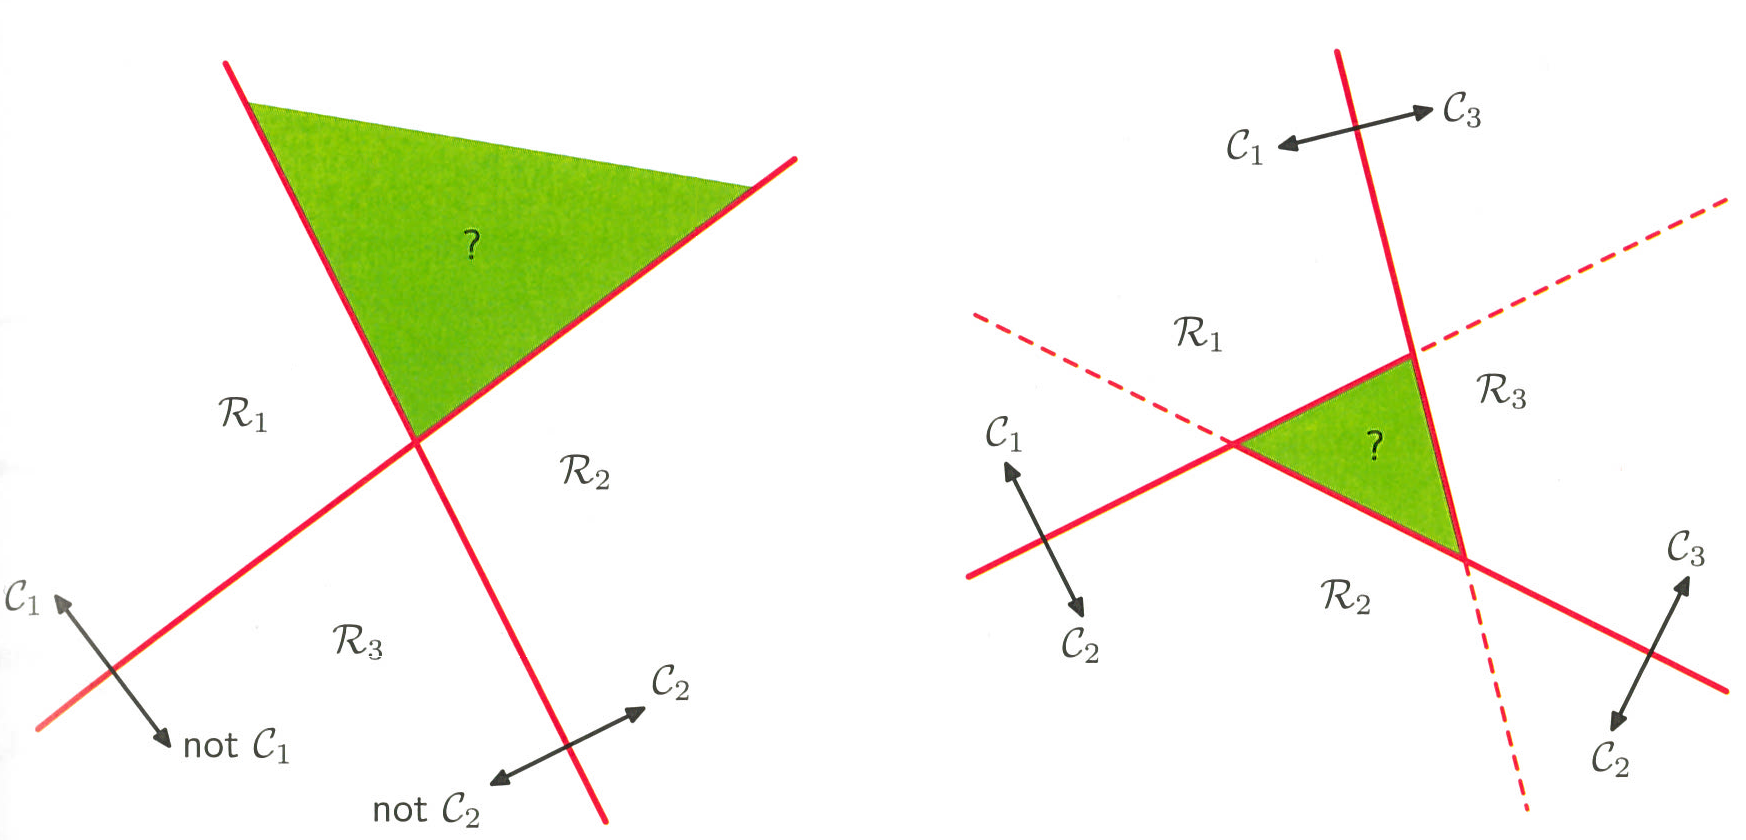
\includegraphics[scale=0.2]{figures/one_vs} 
\newline
\caption{Attempting to construct a $K$ class discriminant from a set of two class discriminants leads to ambiguous regions, shown in green. On the left is an example of \textit{one-versus-the-rest} approach, the discriminant function designed to separate points belonging to a class $C_i$ and points that are not. On the right is an example of \textit{one-versus-all} approach involving 3 discriminant functions, each one separating a pair of classes classes $C_i$ and $C_j$.From: Christopher M. Bishop, \textit{Pattern Recognition and Machine Learning}. Copyright \copyright  2006 by Springer Science.}
\label{one_vs_rest}
\end{center} 
\end{figure}

\noindent An other way to solve a multi-class problem could be to use $\frac{K(K-1)}{2}$ discriminant functions, which is the \textit{one-versus-all} approach. However, the resulting K-class discriminant also has an ambiguous region problem, as seen in Figure \ref{one_vs} \cite{BIS06}.
\newline

\noindent A K-class discriminant which does not lead to an ambiguous region problem is to use K linear discriminant functions $g(x)_k$, $k=1..K$, and to assign an input vector $x$ to a class $C_i$ if $g(x)_i = \max\limits_{k} g_k(x)$. Indeed, as shown in Figure \ref{k_discr}, there are no more ambiguous regions \cite{BIS06}.
\newline

\begin{figure}[!h]
\begin{center}
\noindent 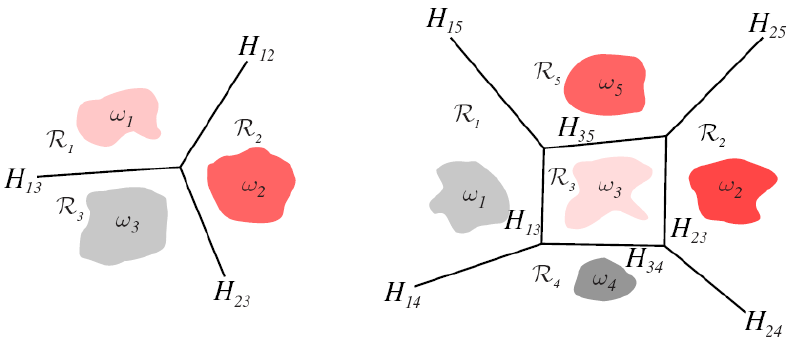
\includegraphics[scale=0.5]{figures/lda_k_disc} 
\newline
\caption{Decision boundaries produced by a linear machine for a 3-class problem and a 5-class problem. From: Richard O. Duda, Peter E. Hart, and David G. Stork, \textit{Pattern Classification}. Copyright \copyright  2001 by John Wiley \& Sons Inc.}
\label{k_disc}
\end{center} 
\end{figure}

\phantomsection
\section{Unsupervised learning}

\vspace{\baselineskip}
\noindent Unlike supervised learning, the classification algorithm is not fed with train data in the case of unsupervised learning. It will be given a set of observable data, and its goal is to group data the smartest way possible, and by itself. Furthermore, in unsupervised learning, the concept of \textit{class} is not applicable any more; the term \textit{cluster} being preferred.
\newline

\noindent The key point of unsupervised algorithms is data clustering. In most common unsupervised algorithms such as K-means, the algorithm can get a hint of the number of clusters it has to find. It then proceeds, usually in an iterative way, to find the latent variables related to the data. Indeed, it is assumed that all observable data is governed by latent variables which can be organized in different levels.
\newline

\noindent Besides K-means, an other common unsupervised algorithm is the Mixture Models algorithm, which will also be described in the following subsections.
\newline

\subsection{K-Means}

\vspace{\baselineskip}
\noindent K-means clustering relies on a set of k reference vectors $\mu_k$, $k=1..K$, also called \textit{prototype vectors}. These vectors represent the centres of the K clusters. This clustering method has two goals: first, it has to find how the clusters are shaped and which data lies in which cluster; secondly, the set of vectors $\{\mu_k\}$ has to be determined while verifying the following condition: for each data point $x_n$, the sum of squares of the distances between $x_n$ and its closest vector $\mu_k$ is a minimum. In other words, equation \ref{distort_fc}, also called \textit{distortion function} has to be minimized \cite{BIS06}.

\begin{equation}
J = \sum\limits_{n=1}\limits^{N} \sum\limits_{k=1}\limits^{K} r_{nk} ||x_n - \mu_k||^2
\label{distort_fc}
\end{equation}

\noindent With

\begin{equation*}
r_{nk} = \left\{
	\begin{array}{ll}
		1 & \mbox{if }  k = arg \min_j ||x_n - \mu_j||^2 \\
		0 & \mbox{otherwise}
	\end{array}
\right.
\end{equation*}
\vspace{\baselineskip}

\noindent This can be achieved through the following iterative algorithm, which result can be seen in Figure \ref{k-mean_res}:
\newline

\begin{algorithmic}
\State Initialization of reference vectors $\mu_k$, $k = 1..K$ 
\Repeat	
	\ForAll{$x_n \in \chi$}
		\State \begin{math} 
			r_{nk} \gets \left\{
			\begin{array}{ll}
				1 & \mbox{if }  k = arg \min_j ||x_n - \mu_j||^2 \\
				0 & \mbox{otherwise}
			\end{array}
			\right.
			\end{math}
	\EndFor
	\ForAll{$\mu_k$, $k = 1..K$ }
		\State $\mu_k \gets \frac{\sum\limits_n r_{nk}x_n}{\sum\limits_n r_{nk}}$
	\EndFor
\Until{$\mu_k$ converge}
\end{algorithmic}

\vspace{\baselineskip}

\begin{figure}[!h]
\begin{center}
\noindent 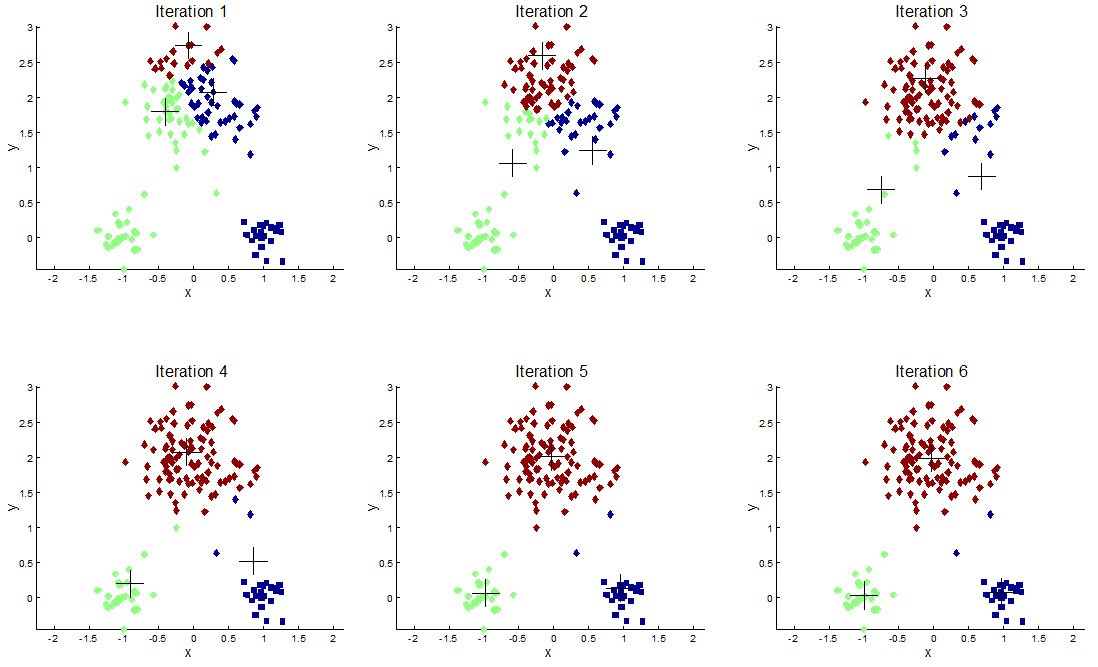
\includegraphics[scale=0.5]{figures/k-mean_res} 
\newline
\caption{Example of application of the iterative K-means algorithm.}
\label{k-mean_res}
\end{center} 
\end{figure}

\noindent In this algorithm, denominator $\sum\limits_n r_{nk}$ corresponds to the number of points assigned to cluster $k$, which sets $\mu_k$ as the mean of the cluster, hence the name \textit{K-means algorithm} \cite{BIS06}.
\newline

\noindent This algorithm can also be used in \textit{lossy data compression}, where input data can be reconstructed with minor errors, in contrary to \textit{lossless data compression}. If the K-means algorithm is applied, then for each data point $x_n$ the only value stored is the cluster $k$ it belongs to. Apart from the data points, values of cluster centres $\mu_k$ are also stored. Hence, during data reconstruction, each data point is approximated by corresponding vector $\mu_k$. This approximation is called \textit{vector quantization} \cite{BIS06}.
\newline

\subsection{Mixture of Gaussians}

\vspace{\baselineskip}
\noindent While the K-means algorithm will try to find reference vectors describing the different clusters, the mixture models algorithm will rather model the underlying distribution of the clusters, usually by a Gaussian probability density function. Each cluster is then represented by a Gaussian distribution, and the aim of the algorithm is to find the best parameters for the latent variables governing these distributions. It can be achieved by finding parameters maximizing likelihood $p(x)=p(x|G_i)p(G_i)$, with:

\begin{itemize}
\item $G_i$: clusters
\item $p(G_i)$: prior probability (mixture proportion)
\item $p(x|G_i)$: component density
\end{itemize}

\noindent Since a Gaussian mixture is roughly similar to $p(x|G_i) \sim \mathcal{N}(\mu_i, \Sigma_i)$, with mean vector $\mu_i$ and covariance matrix $\Sigma_i$, the goal is now to maximize the log likelihood function described in Equation \ref{log_likelihood}.

\begin{equation}
\begin{array}{ll}
\mathcal{L}(\Phi|\chi) & = \ln \prod\limits_n p(x^n | \Phi) \\
 & = \sum\limits_{n=1}\limits^{N} \left\{ \sum \limits_{k=1}\limits^{K} \pi_k \mathcal{N}(x_n|\mu_k, \Sigma_k)\right\}
\end{array}
\label{log_likelihood}
\end{equation}

\noindent with $\Phi$ representing mixing coefficients, including prior probabilities and sufficient statistics of component densities.
\newline

\noindent The maximum likelihood estimation can then be obtained through the \textit{Expectation-Maximization algorithm} for Gaussian Mixture Models (EM), which converges into a result comparable as the one in Figure \ref{mixture_model} \cite{BIS06}.
\newline

\noindent \textbf{Expectation-Maximization algorithm:}
\newline

\begin{algorithmic}
\State Initialize means $\mu_n$, covariances $\Sigma_n$, mixing coefficients $\pi_n$ and compute initial value of the log likelihood

\Repeat
	\State \textbf{Expectation step}: Evaluate the expected value of the latent variable using current parameter values:
		\State $\gamma(z_{nk}) = 
		\frac{\pi_k\mathcal{N}(x_n|\mu_k, \Sigma_k)}{\sum\limits_{j=1}\limits^{K}\pi_j\mathcal{N}(x_n|\mu_j, \Sigma_j)}$
	\State \textbf{Maximization step}: Re-estimate the parameters using $\gamma(z_{nk})$:
		\State $\pi^{new}_k = \frac{N_k}{N}$
		\State $\mu^{new}_k = \frac{1}{N_k}\sum\limits_{n=1}\limits{N}\gamma(z_{nk})x_n$
		\State $\Sigma^{new}_k = \frac{1}{N_k}\sum\limits_{n=1}\limits{N}\gamma(z_{nk}) (x_n - \mu^{new}_k) (x_n - \mu^{new}_k)^T$
		\State Where $N_k = \sum\limits_{n=1}\limits{N}\gamma(z_{nk})$
	\State Evaluate log likelihood $\mathcal{L}$ 
\Until {$\mathcal{L}$ converges}
\end{algorithmic}

\begin{figure}[!h]
\begin{center}
\noindent 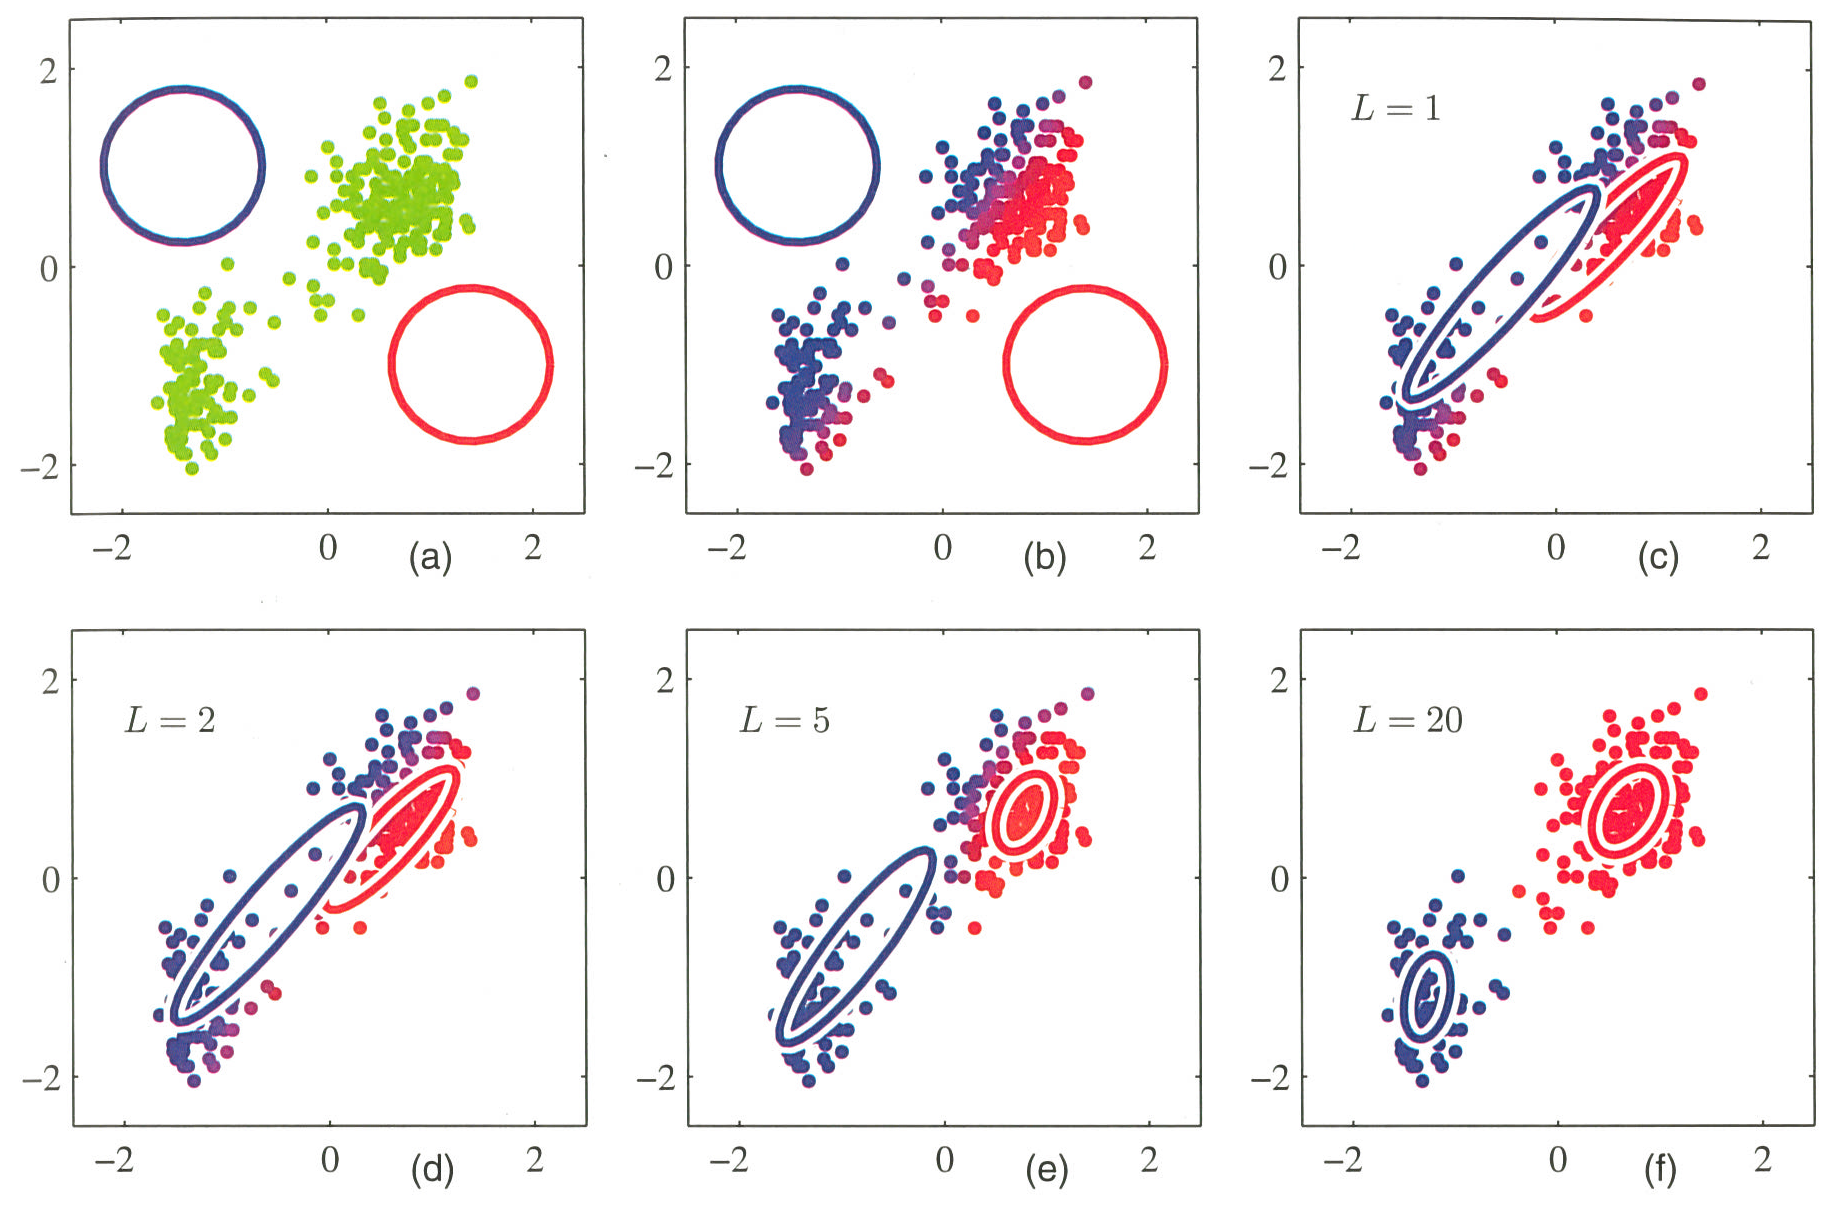
\includegraphics[scale=0.2]{figures/mixture_model} 
\newline
\caption{Illustration of the EM algorithm. From: Christopher M. Bishop, \textit{Pattern Recognition and Machine Learning}. Copyright \copyright  2006 by Springer Science.}
\label{mixture_model}
\end{center} 
\end{figure}
\pagebreak

\newpage
\phantomsection
\chapter{Support Vector Machine}
\label{chap:svm}

\noindent Support Vector Machine (SVM) is a binary linear classifier belonging to the supervised learning algorithms category. It has been proven to be very efficient for classification, regression and novelty detection problems \cite{BIS06}, which makes it suitable for facial expression recognition.
\newline

\noindent This chapter will first provide an overview of how classification is performed using SVM. It will then focus and describe the key points behind this classifier, namely \textit{margin maximization} and \textit{kernel function}. The chapter will conclude with the review of a research paper detailing facial expression recognition using LBP for feature extraction and SVM for classification.
\newline

\phantomsection
\section{Overview}
\label{svm_overview}

\vspace{\baselineskip}
\noindent SVM is originally a binary classifier, which means it has a \textit{one-vs-all} approach. It is a decision machine, so its output is not a posterior probability, but rather a class label \cite{BIS06}.  It can be adapted into a \textit{relevance vector machine} to output posterior probabilities though \cite{BIS06}, but this alternative will not be detailed in our report.
\newline

\noindent SVM is also a linear classifier, such as LDA. For a two-class problem, it will linearly separate the train data by finding the optimal hyperplane between these 2 classes. This hyperplane is defined as being as far as possible from both classes. \textit{Margin maximization} is then applied to optimize the distance between the two classes and the hyperplane, as it will be explained in Section \ref{margin_max}.
\newline

\noindent The name "Support Vector" originates from the margin maximization feature. Indeed, the distance between the classes and the separating hyperplane is computed regarding to the closest data points from both classes. These particular data points, lying on the margins edges, are the support vectors. Some properties are associated to these vectors, such as non-zero Lagrange multipliers (see Section \ref{margin_max}), which builds the classification algorithm.
\newline

\noindent For a multi-class problem, however, this linear separation is not possible anymore. The dataset has to be mapped into an other space, where it can be linearly separated. This is what \textit{kernel functions} are used for, as described in Section \ref{kernel_fct}.
\newline

\phantomsection
\section{Margin maximization}
\label{margin_max}

\vspace{\baselineskip}
\noindent As introduced in Section \ref{svm_overview}, margin maximization for a two-class linear problem starts by finding the separating hyperplane between these two classes. A linear classification model of the form $f(x) = w(x) + b$ can be inferred, with $w$ being the normal to the hyperplane and $b$ the bias. The hyperplane can then be characterized by  $w(x) + b = 0$.
\newline

\noindent Margin is defined as the distance between the closest point of the class to the hyperplane, and that hyperplane, which can also be written as $ d(x) = \frac{|w(x) + b |}{||w||}$. Since a data point $(x_i, y_i)$ is correctly classified if $yf(x) \geq 1$, maximizing the margin is the action of maximizing $||w||^{-1}$, which is consequently equivalent to minimizing $||w||^2$ depending on this constraint. Margin maximization then requires to solve a \textit{quadratic programming} problem under constraints, as seen in Equation \ref{margin_max_eq}.

\begin{equation}
\left\{
\begin{array}{l}
\min \frac{1}{2} ||w||^2 \\
\forall i, \, y_i . f(x) \geq 1
\end{array}
\right.
\label{margin_max_eq}
\end{equation}

\vspace{\baselineskip}

\phantomsection
\section{Kernel function}
\label{kernel_fct}

\vspace{\baselineskip}
\noindent It might however not be possible to perform this linear separation with more classes. Indeed, data might be overlapping, and thus it will not be a linear problem anymore. The solution to overcome this problem is to map the non-linear dataset from its input space into a higher feature space using a function $\Phi(x)$, and perform margin maximization and classification in this higher space. 
\newline

\noindent In order to achieve this mapping, a \textit{kernel function} of the form $K(x_i, x_j) = \Phi(x_i)^T \Phi(x_j)$ is applied to the dataset. This kernel represents an inner product in the feature space. There are four kernels available, which are described in Equation \ref{kernels_svm}.
\newline

\begin{equation}
\begin{array}{ll}
	\text{Linear kernel:} & K(x_i,x_j) = x_i^Tx \\
	\text{Polynomial kernel:} & K(x_i,x_j) = (\gamma x_i^Tx_j + r)^T, \gamma > 0 \\
	\text{Radial Basis Function (Gaussian) kernel:} & K(x_i,x_j) = \exp(-\gamma \| x_i - x_j \|^2), \gamma > 0 \\
	\text{Sigmoid kernel:} & K(x_i,x_j) = \tanh(\gamma x_i^T x_j + r)\\
\end{array}
\label{kernels_svm}
\end{equation}

\noindent The main advantage of using a kernel function is that there is no need to define or calculate $\Phi(x_i)$, only $\Phi(x_i)^T \Phi(x_j)$. We hence do not know the true form of $\Phi(x_i)$. However, simple kernels are usually combined in order to build more complex ones.
\newline

\phantomsection
\section{Combining LBP and SVM}

\vspace{\baselineskip}
\noindent In a 2009 article, Shang and al \cite{SHA09} have performed facial expression recognition while using Local Binary Patterns for feature extraction, and comparing the accuracy of different kinds of classifiers:  template matching,  LDA and SVM. They have used images from the Cohn-Kanade database as train data, and the conclusion of their study is that classification using SVM has a high accuracy rate, as seen in Table \ref{accuracy_svm_lbp}. 
\newline

\begin{table}[h]
   \caption{\label{accuracy_svm_lbp} Recognition performance of LBP-based SVM with different kernels}
\begin{tabular}{|lcc|}
\hline
 & 6-Class recognition (\%) &  7-Class recognition (\%) \\
 \hline
 SVM (linear) & 91.5 $\pm$ 3.1 & 88.1 $\pm$ 3.8 \\
 SVM (polynomial) & 91.5 $\pm$ 3.1 & 88.1 $\pm$ 3.8 \\
 SVM (RBF) & 92.6 $\pm$ 3.1 & 88.9 $\pm$ 3.5 \\
 \hline
\end{tabular}
\end{table}

\noindent Furthermore, as seen in confusion matrices \ref{conf_mtx_6_svm_lbp} and \ref{conf_mtx_7_svm_lbp}, the accuracy for each facial expression is not the same. SVM has some difficulties especially when it comes to distinguish fear and sadness, the two facial expressions which have the lowest accuracy rates. Fear is mistaken with joy, while sadness is mistaken with anger or neutral state. Recognitions rates are however usually better for a 7-class classification, except for fear.
\newline

\noindent Since the accuracy of the system presented in this article is very high, we chose to implement a similar system. Indeed, we are performing facial expression recognition using LBP for feature extraction, and SVM classification. We however did not use the Cohn-Kanade database as train data. We will describe further our implementation and results further in the report. 
\newline

\begin{table}[h]
\caption{\label{conf_mtx_6_svm_lbp} Confusion matrix of 6-class facial expression recognition using SVM (RBF)}
\begin{tabular}{|lcccccc|}
\hline
 & Anger (\%) & Disgust (\%) & Fear (\%) & Joy (\%) & Sadness (\%) & Surprise (\%) \\
\hline
Anger & 89.7 & 2.7 & 0 & 0 & 7.6 & 0 \\
Disgust & 0 & 97.5 & 2.5 & 0 & 0 & 0 \\
Fear & 0 & 2.0 & 73.0 & 22.0 & 3.0 & 0 \\
Joy & 0 & 0.4 & 0.7 & 97.9 & 1.0 & 0 \\
Sadness & 10.3 & 0 & 0.8 & 0.8 & 83.5 & 4.6 \\
Surprise & 0 & 0 & 1.3 & 0 & 0 & 98.7 \\
\hline
\end{tabular}
\end{table}

\begin{table}[h]
\caption{\label{conf_mtx_7_svm_lbp} Confusion matrix of 7-class facial expression recognition using SVM (RBF)}
\begin{tabular}{|lccccccc|}
\hline
& Anger (\%) & Disgust (\%) & Fear (\%) & Joy (\%) & Sadness (\%) & Surprise (\%) & Neutral (\%) \\
\hline
Anger & 85.0 & 2.7 & 0 & 0 & 4.8 & 0 & 7.5 \\
Disgust & 0 & 97.5 & 2.5 & 0 & 0 & 0 & 0 \\
Fear & 0 & 2.0 & 68.0 & 22.0 & 1.0 & 0 & 7.0 \\
Joy & 0 & 0 & 0.7 & 94.7  & 1.1 & 0 & 3.5 \\
Sadness & 8.6 & 0 & 0 & 0 & 69.5 & 2.3 & 19.6 \\
Surprise & 0 & 0 & 1.3 & 0 & 0 & 98.2 & 0.5 \\
Neutral & 1.6 & 0.4 & 0 & 1.6 & 6.0 & 0.4 & 90.0 \\
\hline
\end{tabular}
\end{table}


\stopcontents[parts]



\clearpage
\newpage
\phantomsection
\chapter{Implementation on the Kinect}
\label{chap:implementation_kinect}

\phantomsection
\section{Generalities}
\vspace{\baselineskip}
\noindent The purpose of the project is to implement a system able to recognize emotions through images coming from a Kinect camera sensor. The system is designed to run with Microsoft Windows 7 and need an available USB 2.0 port to plug the Kinect device. The project has been coded in C++, which allows us to include useful third-party libraries in our project.
\newline We used Microsoft Visual Studio 2010 to code and GitHub as a source control management system to facilitate parallel development of features.

\phantomsection
\section{Librairies}
\vspace{\baselineskip}
\noindent Several different libraries have been used to perform facial expression recognition in our system. One for the communication between the computer and Kinect sensors, one for image processing and another one for classification.


\begin{itemize}
  \item The library used for intercommunication with sensors is the Software Development Kit released by Microsoft for their Kinect for XBox in its version 1.0 Beta 2.
  \item OpenCV (Open Source Computer Vision Library) is a graphic library under BSD licence, optimized for real-time image processing. It have been released by Intel and is actually maintained by Willow Garage, a robotic company.
  \item We are using LibSVM to perform classification, which is an OpenSource library for Support Vector Machine. The version used is the 3.14 released on November 16, 2012.
\end{itemize}

\phantomsection
\section{Architecture}

\vspace{\baselineskip}
\noindent The program follow a Model-View-Controller architecture. This MVC pattern consists in 3 modules:

\begin{itemize}
  \item The model part contains all used algorithms;
  \item The view enables user interaction with the system by displaying human-readable information;
  \item The controller sends commands in order to manage the other modules.
\end{itemize}

\noindent Since we use an object-oriented language, the use of the MVC pattern is easier. Five classes have been created: 3 for the architecture, one for LBP processing, and the remaining one for classification, as seen in Figure \ref{uml}.
\newline

\begin{figure}[!h]
\begin{center}
\noindent 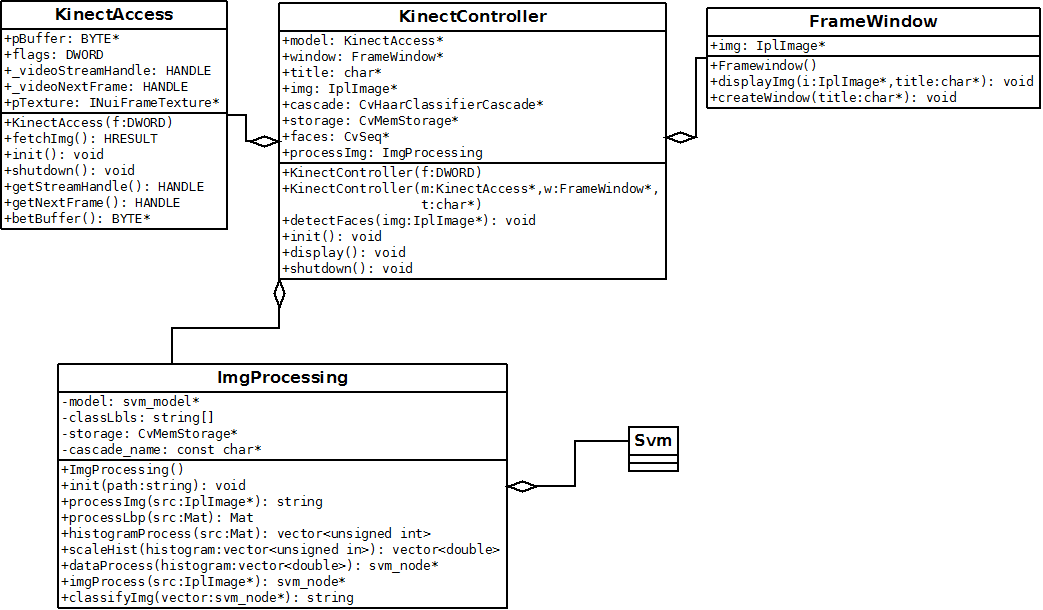
\includegraphics[scale=0.3]{figures/UML} 
\newline
\caption{UML diagram describing our implementation of a facial expression recognition system}
\label{uml}
\end{center} 
\end{figure}

\phantomsection
\section{Interactions}

\vspace{\baselineskip}
\noindent There are two possible ways for the user to interact with the system:
\begin{itemize}
  \item The user has to show a facial expression in front of the camera;
  \item The user has to decide when he or she wants the program to perform facial expression recognition.
\end{itemize}

\noindent The first possibility does not need the user to be active. Indeed, the Kinect camera sensor can record 30 images per second, so each expression can be caught in the image stream. That is why the second possibility needs to be trigged by the user (in our case, press a button) to "capture" the facial expression and start the analysis process. 

\phantomsection
\section{Algorithm}
\vspace{\baselineskip}

\noindent The entry point of the software first initializes the 3 MVC modules. It then runs 3 functions through the controller:

\begin{itemize}
  \item Initialization which loads models (for face detection and classification through SVM) and begins images capture;
  \item Main loop of the program which displays images and waits for actions from the user;
  \item Shutdown process, which deletes models, releases memory and closes communication with sensors.
\end{itemize}

\textbf{Main loop algorithm} 

\begin{algorithmic}
\While{button 'q' is not pressed} 
	\State wait for single object from videoNextFrame handle
	\State result $\gets$ fetchImage(videoStream handle)
	\If{result == success}
		\State Texture $\gets$ Image.texture
		\State LockedRectangle $\gets$ Texture.lockedRectangle
		\If{LockedRectangle.bits $\neq$ 0}
			\State buffer $\gets$ LockedRectangle.bits
			\State unlockRectangle()
			\State releaseImageFrame(videoStream handle)
			\State openCvImage $\gets$ buffer
			\State face $\gets$ detectFace(openCvImage)
			\State roi $\gets$ setRegionOfInterest(face)
			\If{button 'r' is pressed}
				\State openCvImage2 $\gets$ openCvImage
				\State greyscImage $\gets$ convertToGrayscale(openCvImage2)
				\State featVector $\gets$ lbpProcess(greyscIimage)
				\State label $\gets$ classify(featVector)
				\State display(label)
			\EndIf
			\State delete(roi)
		\EndIf
	\EndIf
\EndWhile
\end{algorithmic}



\stopcontents[parts]

%\newpage
  \begin{titlepage}
    \vspace*{\fill}
      \part{Evaluation}
    \vspace*{\fill}
  \end{titlepage}

\startcontents[parts]
  
\phantomsection
\chapter*{Contents}

\textit{This part is two-folded: its first chapter describes the results obtained through this facial expression recognition system, while Chapter~\ref{chap:eval_issues} focuses on the main issues faced when implementing this system. A concluding chapter sums up the framework and methods used in this facial expression recognition system, the results, and explore some possible improvements.} 

\vspace{\baselineskip}

\printcontents[parts]{}{-1}{\setcounter{tocdepth}{1}}

\pagebreak

\phantomsection
\chapter{Results}
\label{chap:eval_results}

\noindent Two kinds of results have been obtained. First results have been obtained by extracting a test set from the KDEF database, and test it against other subjects from the database. Feature extraction is done by LBP, followed by classification using SVM. The second set of results is obtained with the Kinect in real-time conditions, while the entire KDEF database is used for training. The Kinect gets video sequences of a subject in front of it, his or her face being extracted from these sequences using Viola-Jones algorithm. Then the same feature extraction and classification process is applied to these images.
\newline

\phantomsection
\section{First result set}

\vspace{\baselineskip}
\noindent To train the model, 128 face images from the KDEF database have been used for each emotion, plus neutral state. In total, $ 128\times7 = 896 $ face images have been used as train data. To test the system, 12 face images from the KDEF database have been used for each emotion, plus neutral state. In total, $ 12\times7 = 84 $ faces images have been used as test data. For each of these 84 images, face detection was performed first, then the uniform LBP operator extract its features, and then classification is performed using SVM.
\newline

\noindent The model has been trained with different kernels and different parameters. The outcome of these different processes are summed up in Table~\ref{table_results_kernels}.
\newline

\begin{table}[h]
\begin{center}
   \caption{\label{table_results_kernels} Results with different kernels and different parameters}
\begin{tabular}{|c|c|c|c|c|c|c|c|c|}
  \hline
    & Linear & \textbf{Poly1} & Poly2 & RBF1 & RBF2 & Sigmoid1 & Sigmoid2 \\
  \hline
  neutral & 66.00\% & \textbf{83.33\%} & 83.33\% & 83.33\% & 66.67\% & 8.33\% & 66.67\% \\
  afraid & 58.33\% & \textbf{83.33\%} & 75.00\% & 66.67\% & 66.67\% & 66.67\% & 58.33\% \\
  angry & 41.67\% & \textbf{41.67\%} & 33.33\% & 50.00\% & 41.67\% & 16.67\% & 41.67\% \\
  disgusted & 58.33\% & \textbf{75.00\%} & 75.00\% & 50.00\% & 50.00\% & 16.67\% & 58.33\% \\
  happy & 100.00\% & \textbf{100.00\%} & 91.67\% & 91.67\% & 100.00\% & 66.67\% & 100.00\% \\
  sad & 8.33\% & \textbf{8.33\%} & 0.00\% & 8.33\% & 8.33\% & 8.33\% & 8.33\% \\
  surprised & 66.67\% & \textbf{75.00\%} & 75.00\% & 66.67\% & 66.67\% & 25.00\% & 66.67\% \\
  \textbf{overall} & \textbf{57.14\%} & \textbf{{\color{red}66.67\%}} & \textbf{61.90\%} & \textbf{59.52\%} & \textbf{57.14\%} & \textbf{29,76\%} & \textbf{57.14\%} \\
  \hline
\end{tabular}
\end{center} 
\end{table}

\noindent \textit{Poly1} stands for Polynomial and has degree parameter: $ D = 2 $ and $ \gamma = 0.001953125 $
\newline
\noindent \textit{Poly2} stands for Polynomial and has degree parameter: $ D = 3 $ and $ \gamma = 0.001953125 $
\newline
\noindent \textit{RBF1} has cache and $\gamma$ parameters: $ C = 128 $ and $ \gamma = 0.0078125 $
\newline
\noindent \textit{RBF2} has cache and $\gamma$ parameters: $ C = 8192 $ and $ \gamma = 0.00048828125 $ 
\newline
\noindent \textit{Sigmoid1} has cache and $\gamma$ parameters: $ C = 128 $ and $ \gamma = 0.0078125 $
\newline
\noindent \textit{Sigmoid2} has cache and $\gamma$ parameters: $ C = 8192 $ and $ \gamma = 0.00048828125 $
\newline

\noindent As said in Chapter \ref{chap:implementation_svm}, parameters for RBF and sigmoid kernels are found by the \textit{gridsearch} script of LIBSVM. For the polynomial kernel, as said in Chapter \ref{chap:implementation_svm}, the degree parameter $D$ has to be chosen, otherwise the default value is $D=3$. \textit{Poly2} has default $D$ value, while \textit{Poly1} has $D = 2$. It has been chosen because if the dimension is superior to $3$ then there an \textit{overfitting} issue. It means that the model yields good results, not because it has been trained with suitable parameters, but because it fits the test data too much, and will have erroneous results if given other data.
\newline

\noindent A model has also been trained with same kernels and parameters but using cross-validation (as explained in Chapter \ref{chap:implementation_svm}). Results obtained with a model using cross-validation are compared to those with a model trained normally, this comparison being shown in  Table~\ref{table_results_crossvalidation}. All results are inferior or equal to those without cross-validation, except for the sigmoid kernel tuned with parameters cache and $\gamma$ equals to $ C = 8192 $ and $ \gamma = 0.00048828125 $.
\newline

\begin{table}[h]
\begin{center}
   \caption{\label{table_results_crossvalidation} Results with and without cross validation}
\begin{tabular}{|c|c|c|c|c|c|c|c|c|}
  \hline
    & with cross validation & without cross validation \\
  \hline
  Linear & 57.14\% & 57.14\% \\
  Poly1 & 55.95\% & 66.67\% \\
  Poly2 & 47.62\% & 61.90\% \\
  RBF1 & 52.52\% & 59.52\% \\
  RBF2 & 55.95\% & 57.14\% \\
  Sigmoid1 & 16.67\% & 29,76\% \\
  Sigmoid2 & 63.10\% & 57.14\% \\
  \hline
\end{tabular}
\end{center}
\end{table}

\noindent The best accuracy percentage is for a model trained with Poly1 kernel parameters, with an overall accuracy rate of$ 66.67\% $. It is obtained with a classification based on the polynomial kernel and with following parameters: $ D = 2 $ and $ \gamma = 0.001953125 $. Table~\ref{table_results_confusion_matrix} represents the confusion matrix for this kernel.
\newline

\begin{table}[h]
\begin{center}
   \caption{\label{table_results_confusion_matrix} Confusion matrix}
\begin{tabular}{|c|c|c|c|c|c|c|c|c|}
  \hline
   & neutral & afraid & angry & disgusted & happy & sad & surprised & accuracy \\
  \hline
  neutral & \textbf{10} & 0 & 0 & 0 & 0 & 2 & 0 & 83.33\% \\
  afraid & 0 & \textbf{10} & 1 & 0 & 0 & 0 & 1 & 83.33\% \\
  angry & 4 & 0 & \textbf{5} & 0 & 0 & 3 & 0 & 41.67\% \\
  disgusted & 1 & 0 & 0 & \textbf{9} & 1 & 1 & 0 & 75.00\% \\
  happy & 0 & 0 & 0 & 0 & \textbf{12} & 0 & 0 & 100.00\% \\
  sad & 5 & 1 & 2 & 2 & 1 & \textbf{1} & 0 & 8.33\% \\
  surprised & 0 & 3 & 0 & 0 & 0 & 0 & \textbf{9} & 75.00\%\\
  \hline
\end{tabular}
\end{center}
\end{table}

\noindent By looking at the confusion matrix, it is easy to notice that 2 facial expressions are harder to recognize than others with this system: \textit{angry} and \textit{sad}. There is a great difference between these 2 emotions and the 5 other ones (afraid, disgusted, happy, neutral and surprised). Indeed, these 2 emotions are recognized with an accuracy lower than $ 50\% $, while the 4 other ones are recognized with an accuracy equal or higher than $ 75\% $, as summed up in Table~\ref{table_results_accuracy}. Furthermore, the recognition accuracy for the \textit{sad} expression is much lower than random guess, which really contrasts with the \textit{happy} facial expression, the latter reaching a $100\%$ accuracy.
\newline

\begin{table}[h]
\begin{center}
   \caption{\label{table_results_accuracy} Recognition accuracy of the six basic emotions and of the neutral state}
\begin{tabular}{|c|c|c|c|c|c|c|c|c|}
  \hline
   $ < 50\% $ & > 75\% \\
  \hline
  angry ($ 5/12 $) & afraid ($ 10/12 $) \\
  sad ($ 1/12 $) & disgusted ($ 9/12 $) \\
   & happy ($ 12/12 $) \\
   & surprised ($ 9/12 $) \\
   & neutral ($ 10/12 $) \\
  \hline
\end{tabular}
\end{center} 
\end{table}

\noindent The numbers in parenthesis represent the number of faces correctly classified over the total number of face images tested.
\newline

\noindent These 6 emotions plus the neutral state can be categorized into 2 groups. Indeed, one group containing the 2 emotions hard to recognize and another group containing the 5 remaining emotions.
\newline

\noindent The first group contains the 5 following facial expressions \textit{afraid}, \textit{disgusted}, \textit{happy}, \textit{surprised} and the \textit{neutral} state. These emotions distort significantly the face when they are expressed except for the neutral state that is the basic face of the subject when he does not express an emotion. This is why it is easier to recognize them. Figure~\ref{kdef_difference_emotions} shows face images from the KDEF database used in the test set, expressing these 5 facial expressions. Important features carrying emotion as the mouth or the eyes are changing a lot while these 5 emotions are expressed.
\newline

\begin{figure}[!h]
\begin{center}
\noindent 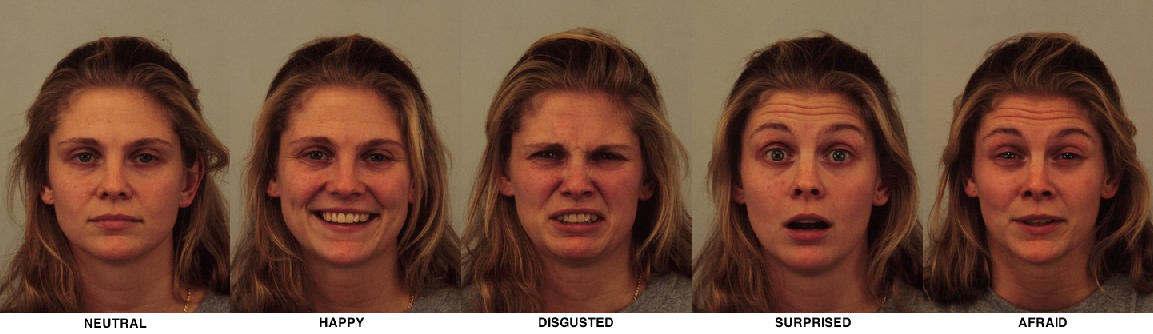
\includegraphics[scale=0.3]{figures/kdef_difference_emotions} 
\newline
\caption{Face images from the KDEF database used in the test set}
\label{kdef_difference_emotions}
\end{center} 
\end{figure}

\noindent As it can be seen in Figure~\ref{kdef_difference_emotions}, for each emotion, eyebrows are raised, eyes are widely opened, and the mouth has a distinct shape, whereas in Figure~\ref{kdef_no_difference_emotions} there are no differences as visible as in Figure~\ref{kdef_difference_emotions}. These variations of intensity might explain why the system struggles when trying to differentiate \textit{angry} and \textit{sad} emotional states.
\newline

\noindent The second group contains the 2 remaining facial expressions. The 2 facial expressions \textit{angry} and \textit{sad}, are the ones that distort the less the face. For a same subject expressing these 2 different emotions, as in Figure~\ref{kdef_no_difference_emotions}, the differences are not clearly noticeable.
\newline

\begin{figure}[!h]
\begin{center}
\noindent 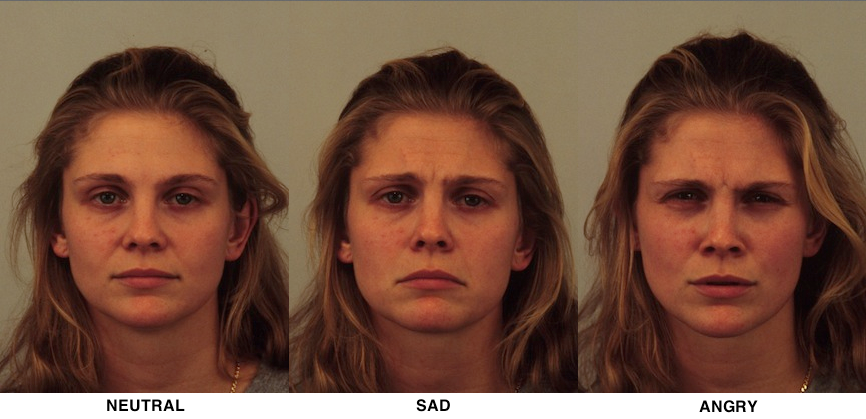
\includegraphics[scale=0.3]{figures/kdef_no_difference_emotions} 
\newline
\caption{Face images from the KDEF database used in the test set}
\label{kdef_no_difference_emotions}
\end{center} 
\end{figure}

\noindent The \textit{sad} emotion is the one that is the hardest to recognize. On 12 times, it has been well recognized only once. It is mostly taken for the \textit{neutral} state. As it can be seen in the Figure~\ref{kdef_no_difference_emotions}, there is not clear change between the \textit{neutral} state and the \textit{sad} emotion. Only the eyebrows are lightly frowned.
\newline

\noindent The \textit{angry} emotion is also hard to recognize. On 12 times, it has been well recognized only 5 times. It is mostly taken for the \textit{neutral} state and for the \textit{angry} emotion. As it can be seen in the Figure~\ref{kdef_no_difference_emotions}, there is not clear change between the \textit{neutral} state, the \textit{sad} emotion and the \textit{angry} emotion. Only the eyebrows slightly change as the eyes. The mouth is almost identical between the three face images in the Figure~\ref{kdef_no_difference_emotions}
\newline

\phantomsection
\section{Second result set}

\vspace{\baselineskip}
\noindent The second result test is processed in the same way as the first data set, the only difference being the input. Indeed, it is not performed on static images extracted from the KDEF database anymore; images used for texting are extracted from the video stream coming from the Kinect. A subject stands in front of the Kinect, his or her face is detected and extracted, then features are computed, and finally classification is performed. It runs almost in real-time, and the process outputs the name of the emotion expressed.
\newline

\subsection{With face images from the KDEF database}

\vspace{\baselineskip}
\noindent Because the results do not have a good accuracy at first sight, another method is tested. Face images from the KDEF database are given as input directly to our program. This way the data can be tested. Ten face images are randomly chosen among all the face images present in the KDEF database to be tested for each emotion. 
\newline

\noindent The model used is the one that gave the best results in the first test set: polynomial kernel with following parameters: $ D = 2 $ and $ \gamma = 0.001953125 $. Table~\ref{table_results_confusion_matrix_offline} represents the confusion matrix for this kernel and these test conditions.
\newline

\begin{table}[h]
\begin{center}
   \caption{\label{table_results_confusion_matrix_offline} Confusion matrix}
\begin{tabular}{|c|c|c|c|c|c|c|c|c|}
  \hline
   & neutral & afraid & angry & disgusted & happy & sad & surprised & accuracy \\
  \hline
  neutral & \textbf{6} & 1 & 2 & 0 & 0 & 1 & 0 & 60.00\% \\
  afraid & 0 & \textbf{4} & 0 & 3 & 0 & 3 & 0 & 40.00\% \\
  angry & 2 & 1 & \textbf{6} & 1 & 0 & 0 & 0 & 60.00\% \\
  disgusted & 0 & 1 & 0 & \textbf{7} & 1 & 1 & 0 & 70.00\% \\
  happy & 0 & 0 & 0 & 0 & \textbf{10} & 0 & 0 & 100.00\% \\
  sad & 1 & 3 & 2 & 1 & 1 & \textbf{2} & 0 & 20.00\% \\
  surprised & 0 & 0 & 0 & 0 & 0 & 0 & \textbf{10} & 100.00\%\\
  \hline
\end{tabular}
\end{center}
\end{table}

\noindent The overall accuracy rate is of $ 64.28\% $ which is lower than the one obtained in the first result set: $ 66.67\% $. The results obtained are consistent with the ones found in the first result set.
\newline

\subsection{With subjects}

\vspace{\baselineskip}
\noindent For this test set, we use face images from the JAFFE database that are placed in front of the Kinect. Ten face images has been chosen randomly from this databases for each emotion.
\newline

\noindent As for the precedent part, the model used is the polynomial kernel with the following parameters: $ D = 2 $ and $ \gamma = 0.001953125 $. Table~\ref{table_results_confusion_matrix_kinect} represents the confusion matrix for this kernel and these test conditions.
\newline

\begin{table}[h]
\begin{center}
   \caption{\label{table_results_confusion_matrix_kinect} Confusion matrix}
\begin{tabular}{|c|c|c|c|c|c|c|c|c|}
  \hline
   & neutral & afraid & angry & disgusted & happy & sad & surprised & accuracy \\
  \hline
  neutral & \textbf{6} & 0 & 0 & 0 & 0 & 4 & 0 & 60.00\% \\
  afraid & 2 & \textbf{1} & 1 & 0 & 0 & 6 & 0 & 10.00\% \\
  angry & 3 & 0 & \textbf{0} & 0 & 0 & 7 & 0 & 0.00\% \\
  disgusted & 1 & 0 & 1 & \textbf{0} & 0 & 8 & 0 & 0.00\% \\
  happy & 4 & 3 & 0 & 0 & \textbf{0} & 3 & 0 & 0.00\% \\
  sad & 4 & 0 & 0 & 0 & 0 & \textbf{5} & 1 & 50.00\% \\
  surprised & 5 & 0 & 1 & 0 & 0 & 4 & \textbf{0} & 0.00\%\\
  \hline
\end{tabular}
\end{center}
\end{table}

\noindent The overall accuracy rate is of $ 15,71\% $ which is really low compared to the precedent result that is of $ 64.28\% $  and to the one obtained in the first result set that is of $ 66.67\% $. The results obtained are consistent with the ones found in the first result set.
\newline

\phantomsection
\section{Additional results}

\vspace{\baselineskip}
\noindent One way to obtain better results with the LBP operator for this system is to add weights for each of the 42 regions of the face, as seen in Chapter~\ref{chap:lbp}. The LBP operator used in this system is already far from the basic LBP operator; it is a uniform circular LBP operator. Even though the results obtained with this operator are quite good with an accuracy of $ 66.67\% $, there is still room for improvement. Weighting the regions of the face will have an impact on the computed histogram, hence on the resulting feature vector ready for classification. \newline

\noindent The face image is divided in 42 regions ($ 7 $ rows $\times$ $ 6 $ columns), as seen in Chapter~\ref{chap:lbp}, and mentioned in \cite{GAN08}. The weights are however not applied in the same way as in \cite{GAN08}, but rather as in Figure~\ref{lbp_region_weight}. Figure~\ref{implementation_weight_example} shows an example of the division into regions of face images from the KDEF database that this system uses. Thus, border regions are less important than those containing the ROI of the face (eyes, nose, mouth). Figure~\ref{implementation_weight_example} shows an example of the division into regions of face images from the KDEF database used by this system.
\newline

\begin{figure}[!h]
\begin{center}
\noindent 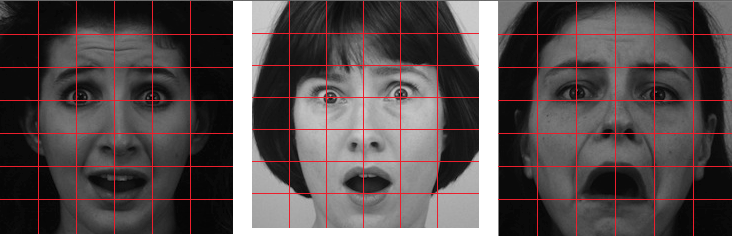
\includegraphics[scale=0.3]{figures/implementation_weight_example} 
\newline
\caption{Example of division into regions of face images from the KDEF database}
\label{implementation_weight_example}
\end{center} 
\end{figure}

\noindent Results has been obtained using the same process than for the first set result. The results with the weights applied are summed up in Table~\ref{table_results_kernels_weight}. The model has been trained with cross validation.
\newline

\begin{table}[h]
\begin{center}
   \caption{\label{table_results_kernels_weight} Results with different kernels and different parameters}
\begin{tabular}{|c|c|c|c|c|c|c|c|c|}
  \hline
    & Linear & \textbf{Poly1} & Poly2 & RBF1 & RBF2 & Sigmoid1 & Sigmoid2 \\
  \hline
  neutral & 75.00\% & 75.00\% & 91,67\% & \textbf{91,67\%} & 75.00\% & 100.00\% & 66.67\% \\
  afraid & 91,67\% & 83.33\% & 100.00\% & \textbf{100.00\%} & 83.33\% & 33.33\% & 91,67\% \\
  angry & 58.33\% & 58.33\% & 41.67\% & \textbf{66.67\%} & 58.33\% & 50.00\% & 50.00\% \\
  disgusted & 41.67\% & 58.33\% & 50.00\% & \textbf{50.00\%} & 50.00\% & 75.00\% & 41.67\% \\
  happy & 100.00\% & 100.00\% & 91.67\% & \textbf{100.00\%} & 100.00\% & 91.67\% & 91.67\% \\
  sad & 8.33\% & 8.33\% & 8.33\% & \textbf{8.33\%} & 8.33\% & 8.33\% & 8.33\% \\
  surprised & 75.00\% & 75.00\% & 75.00\% & \textbf{83.33\%} & 75.00\% & 66.67\% & 75.00\% \\
  \textbf{overall} & \textbf{64.29\%} & \textbf{65.48\%} & \textbf{{65.48\%}\%} & \textbf{{\color{red}71.42\%}} & \textbf{64.29\%} & \textbf{59.52\%} & \textbf{60.71\%} \\
  \hline
\end{tabular}
\end{center} 
\end{table}

\noindent \textit{Poly1} stands for Polynomial and has degree parameter: $ D = 2 $ and $ \gamma = 0.001953125 $
\newline
\noindent \textit{Poly2} stands for Polynomial and has degree parameter: $ D = 3 $ and $ \gamma = 0.001953125 $
\newline
\noindent \textit{RBF1} has cache and $\gamma$ parameters: $ C = 128 $ and $ \gamma = 0.0078125 $
\newline
\noindent \textit{RBF2} has cache and $\gamma$ parameters: $ C = 8192 $ and $ \gamma = 0.00048828125 $ 
\newline
\noindent \textit{Sigmoid1} has cache and $\gamma$ parameters: $ C = 128 $ and $ \gamma = 0.0078125 $
\newline
\noindent \textit{Sigmoid2} has cache and $\gamma$ parameters: $ C = 8192 $ and $ \gamma = 0.00048828125 $
\newline

\noindent A model has also been trained with same kernels and parameters but without cross-validation. Comparison has been made between the model with cross validation and the one without cross validation as it is shown in  Table~\ref{table_results_crossvalidation_weight}. Sometimes results are better with cross validation, sometimes results are better without it. The best result however is obtained with cross validation.
\newline

\begin{table}[h]
\begin{center}
   \caption{\label{table_results_crossvalidation_weight} Results with and without cross validation}
\begin{tabular}{|c|c|c|c|c|c|c|c|c|}
  \hline
    & with cross validation & without cross validation \\
  \hline
  Linear & 64.29\% & 66.67\% \\
  Poly1 & 65.48\% & 65.48\% \\
  Poly2 & 65.48\% & 65.48\% \\
  RBF1 & 71.42\% & 63.10\% \\
  RBF2 & 64.29\% & 67.86\% \\
  Sigmoid1 & 59.52\% & 60.71\% \\
  Sigmoid2 & 60.71\% & 67.86\% \\
  \hline
\end{tabular}
\end{center}
\end{table}

\noindent The best accuracy percentage is for a model trained with RBF1 kernel parameters and with cross validation, with an overall accuracy rate of$ 71.42\% $. It is obtained with a classification based on the RBF kernel and with following parameters: $ C = 128 $ and $ \gamma = 0.0078125 $. Table~\ref{table_results_confusion_matrix_weight} represents the confusion matrix for this kernel.
\newline

\begin{table}[h]
\begin{center}
   \caption{\label{table_results_confusion_matrix_weight} Confusion matrix}
\begin{tabular}{|c|c|c|c|c|c|c|c|c|}
  \hline
   & neutral & afraid & angry & disgusted & happy & sad & surprised & accuracy \\
  \hline
  neutral & \textbf{11} & 0 & 0 & 0 & 0 & 1 & 0 & 91.67\% \\
  afraid & 0 & \textbf{12} & 0 & 0 & 0 & 0 & 0 & 100.00\% \\
  angry & 2 & 0 & \textbf{8} & 0 & 1 & 1 & 0 & 66.67\% \\
  disgusted & 1 & 2 & 1 & \textbf{6} & 2 & 0 & 0 & 50.00\% \\
  happy & 0 & 0 & 0 & 0 & \textbf{12} & 0 & 0 & 100.00\% \\
  sad & 2 & 8 & 1 & 0 & 0 & \textbf{1} & 0 & 8.33\% \\
  surprised & 0 & 2 & 0 & 0 & 0 & 0 & \textbf{10} & 83.33\%\\
  \hline
\end{tabular}
\end{center}
\end{table}

\noindent As for the first test result, two emotions are hard for our system to recognize: the \textit{sad} emotion and the \textit{disgusted} emotion (see Table~\ref{table_results_accuracy_weight}). But this time this is not the \textit{angry} emotion that has bad results but the \textit{disgusted} emotion.
\newline

\begin{table}[h]
\begin{center}
   \caption{\label{table_results_accuracy_weight} Recognition accuracy of the six basic emotions and of the neutral state}
\begin{tabular}{|c|c|c|c|c|c|c|c|c|}
  \hline
   $ \leq 50\% $ & > 66.67\% \\
  \hline
  disgusted ($ 6/12 $) & afraid ($ 12/12 $) \\
  sad ($ 1/12 $) & angry ($ 8/12 $) \\
   & happy ($ 12/12 $) \\
   & surprised ($ 10/12 $) \\
   & neutral ($ 11/12 $) \\
  \hline
\end{tabular}
\end{center} 
\end{table}

\noindent Once again the \textit{sad} emotion is the one getting really bad results. However, with the weights applied to each region, better results are obtained. The percentage of accuracy is of $71.42\%$ instead of $66.67\%$ without the weights applied.
\newline

\newpage
\phantomsection
\chapter{Issues}
\label{chap:eval_issues}

\phantomsection
\section{Feature extraction}

\vspace{\baselineskip}
\noindent The feature extraction method chosen for this facial expression recognition system is the Local Binary Patterns method. As seen in chapter~\ref{chap:lbp}, there are many ways to improve the basic LBP operator. This ways can be using the circular LBP operator, using the uniform LBP operator or applying weights to each region of the face image. The basic LBP operator is quite simple but after improving it at its best, it requires more computation time but gives better result.
\newline

\noindent The LBP operator used in this system has already some improvements; it is a uniform circular LBP operator. The results obtained with this operator are quite good with an accuracy of $ 61.90\% $. But this percentage of accuracy can be improved by weighting each region of the face for example. This system has trouble recognizing some of the 7 emotions; more particularly the \textit{sad} emotion.
\newline

\noindent The Local Binary Patterns method was chosen because the LBP operator gives good results and has a discriminative power, and because the basic LBP operator is simple (and it can be improved in many ways). But there are most likely other methods that give equal results to the ones of the LBP operator or even better results. There are also certainly other methods that are more optimized than the LBP operator and that take less computation time. Even if the LBP operator seems to be a good compromise between computation time and results; other methods can be implemented to compare the performance of each algorithm with the same test conditions.
\newline

\phantomsection
\section{Real-time}

\vspace{\baselineskip}
\noindent The computation of the LBP operator takes about 1-4 seconds (depending on the computer). It was not expected that it takes so long. it was more expected to obtain a computation time on the order of milliseconds. That is why this facial expression recognition system does not really work in real-time an why it needs an interaction with the subject. With the Kinect, 30 frames are received per second. The system should take 33,3 milliseconds maximum ($ \frac{1}{30} = 0,0333 s $) so that it could work in real-time and have the time to process each frame. 
\newline

\noindent The basic LBP operator is quite simple so a system based on this feature extraction method should be able to work in real-time. Using the circular LBP operator adds some computation time; but the use of the uniform LBP allows to reduce the computation time by only considering the uniform LBP and not the non-uniform ones.
\newline

\noindent The system was adapted so that it can still work with video sequences and almost in real-time. The subject stands in front of the Kinect and express an emotion among the 6 basic ones plus the neutral one. When the subject thinks that the emotion that is expressed is good, then he can click on the interface to launch the processing with this exact face he made. Then only one frame is used, the one he chose when he clicked. This frame is processed and classified and the output given to the subject is the name of the emotion that he expressed. The output is given about 2 seconds after the subject's click.
\newline

\phantomsection
\section{Training dataset}

\vspace{\baselineskip}

\noindent bla bla bla
\newline
\newpage
\phantomsection
\chapter{Conclusion}
\label{chap:ccl}
  
\phantomsection
\section{Theoretical framework}

\vspace{\baselineskip}
\noindent The theoretical framework on which this system is based relies on three major points: face detection, feature extraction and classification. Face detection is achieved through Viola-Jones face detection algorithm. This cascade of AdaBoost classifiers based on Haar-like features results in a strong binary classifier, composed of a chain of small weak ones. Moreover, the use of integral images enables real-time detection.
\newline

\noindent Feature extraction is performed using Local Binary Patterns, a simple but efficient texture descriptor encoding changes in micro-patterns. It outputs histograms which bin indexes are intensity values of the pixels, and bin sizes the number of pixels having this value. This texture descriptor can be used for facial feature extraction, and can be modified in order to detect patterns of various sizes and shapes, but also to reduce histogram size, hence improving computation time.
\newline

\noindent Thirdly, Support Vector Machine is used as classifier. This binary linear classifier, belonging to the supervised learning category, is based on \textit{margin maximization} and \textit{kernel functions}. Indeed, since it is a linear classifier, data has to be mapped into a higher space for the classifier to perform correctly. Four classic kernels can be used, and even combined if needed. When compared to other classification methods, SVM yields better results, which makes it a suitable choice for facial expression recognition using Local Binary Patterns.
\newline

\phantomsection
\section{Results}

\vspace{\baselineskip}
\noindent Different results are obtained based on the use of the Kinect or not.
\newline

\noindent Results obtained by using face images of the KDEF database as test set are quite good, with an accuracy rate of $ 66.67\% $. There is nevertheless an issue with the \textit{sad} emotion, which stands out because of its bad recognition accuracy. This emotion is mostly misclassified as \textit{neutral} state. Indeed these two emotions are quite similar, almost identical when it comes to feature extraction, hence the low accuracy rate.
\newline

\noindent The \textit{angry} emotion also has a below average recognition accuracy, but it is not as significant as for the \textit{sad} emotion. The reason behind this result is the same as for the \textit{sad} emotion. Since an \textit{angry} face is more distorted than a \textit{sad} face it is more easily classified correctly. The accuracy rate is thus of $ 41.67\% $ for the \textit{angry} expression,  instead of $ 8.33\% $ for \textit{sad}.
\newline

\noindent Concerning results obtained with the Kinect, the accuracy rate is significantly lower.
\newline

\phantomsection
\section{Improvements}

\subsection{Local Binary Patterns}

\vspace{\baselineskip}
\noindent One of the way to improve the LBP operator of this system is to add weights for each of the 42 regions of the face, as seen in Chapter~\ref{chap:lbp}. The LBP operator used in this system is already far from the basic LBP operator; it is a uniform circular LBP operator. Even though the results obtained with this operator are quite good with an accuracy of $ 66.67\% $, there is still room for improvement. Weighting the regions of the face will have an impact on the computed histogram, hence on the resulting feature vector ready for classification. \newline

\noindent The face image is divided in 42 regions ($ 7 $ rows $\times$ $ 6 $ columns), as seen in Chapter~\ref{chap:lbp}, and mentioned in \ref{GAN08}. The weights are however not applied in the same way as in \ref{GAN08}, but rather as in Figure~\ref{lbp_region_weight}. Figure~\ref{implementation_weight_example} shows an example of the division into regions of face images from the KDEF database that this system uses. Thus, border regions are less important than those containing the ROI of the face (eyes, nose, mouth). Figure~\ref{implementation_weight_example} shows an example of the division into regions of face images from the KDEF database used by this system.
\newline

\begin{figure}[!h]
\begin{center}
\noindent 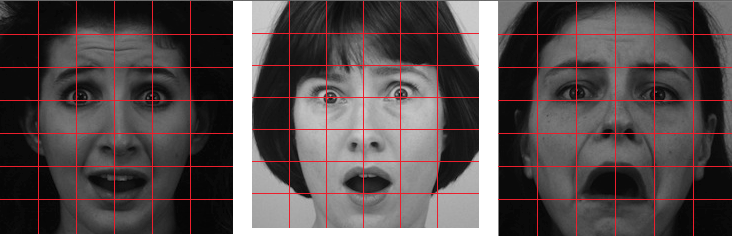
\includegraphics[scale=0.3]{figures/implementation_weight_example} 
\newline
\caption{Example of division into regions of face images from the KDEF database}
\label{implementation_weight_example}
\end{center} 
\end{figure}

\noindent GIVE RESULTS WITH WEIGHTS APPLIED
\newline

\noindent Another way to improve the LBP operator would be to use one with larger scale, hence modify the radius of the circular operator; for example, $ LBP_{12,2.5}^{u^2} $ or $ LBP_{16,4.0}^{u^2} $ (with $ P = 12 $ and $ R = 2.5 $ or with $ P = 16 $ and $ R = 4.0 $). This implies to use the bilinear interpolation because sampling points do not fall exactly on pixels, as seen in Chapter~\ref{chap:lbp}. However, using bilinear interpolation is more computationally expensive. A good compromise has to be found between computation time and accuracy rate.
\newline

\subsection{Combination of feature extraction methods}

\vspace{\baselineskip}
\noindent To improve the accuracy of LBP feature extraction method, another feature extraction method can be used and combined with it. 
\newline

\noindent  For example, a method has been proposed by Liao et al. \cite{LIA09}, where they combine LBP and Gabor filter. It is called Dominant Local Binary Patterns (DLBP), and is robust against change of lighting, image rotation and image noise.  It works by using the most recurrent patterns of the LBP method to obtain more information on the texture. It also uses the Gabor method to add global texture information to one already obtained by LBP. It works based on the circularly symmetric Gabor filter responses \cite{LIA09}. Figure~\ref{combination_lbp_gabor} contains two face images of the YaleB face database , and shows the robustness of the combination against change in lighting. Image (a) is the original image with different lighting conditions, and image (b) is the preprocessed image with the Gabor wavelets. Image (c) is the same image, mapped with the LBP operator. Finally, image (d) is the preprocessed image with the combination of the two methods \cite{GOH11}.
\newline

\begin{figure}[!h]
\begin{center}
\noindent 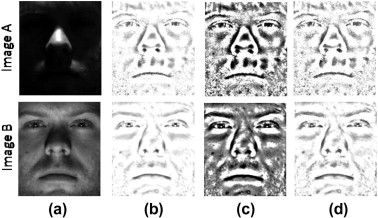
\includegraphics[scale=1]{figures/combination_lbp_gabor} 
\newline

\caption{2 face images of the YaleB face database (a) when processed with Gabor wavelets (b), LBP (c), and Gabor wavelets+LBP (d)\cite{GOH11}}
\label{combination_lbp_gabor}
\end{center} 
\end{figure}

\noindent  LBP has also been combined with the Scale Invariant Feature Transform descriptor (SIFT), which is a ROI descriptor. This descriptor is robust against image rotation, image translations, scaling and lighting variations. Heikkila et al. introduced a combination of the SIFT descriptor with the LBP operator \cite{HEI09}.
\newline


\stopcontents[parts]
\hypersetup{bookmarksdepth=0} 
\bookmarksetup{startatroot}% faire en sorte que la conclusion ne soit pas incluse dans la partie précédente
\addtocontents{toc}{\bigskip}
\cleardoublepage
\phantomsection
\chapter{Conclusion}
\label{chap:ccl}
  
\phantomsection
\section{Theoretical framework}

\vspace{\baselineskip}
\noindent The theoretical framework on which this system is based relies on three major points: face detection, feature extraction and classification. Face detection is achieved through Viola-Jones face detection algorithm. This cascade of AdaBoost classifiers based on Haar-like features results in a strong binary classifier, composed of a chain of small weak ones. Moreover, the use of integral images enables real-time detection.
\newline

\noindent Feature extraction is performed using Local Binary Patterns, a simple but efficient texture descriptor encoding changes in micro-patterns. It outputs histograms which bin indexes are intensity values of the pixels, and bin sizes the number of pixels having this value. This texture descriptor can be used for facial feature extraction, and can be modified in order to detect patterns of various sizes and shapes, but also to reduce histogram size, hence improving computation time.
\newline

\noindent Thirdly, Support Vector Machine is used as classifier. This binary linear classifier, belonging to the supervised learning category, is based on \textit{margin maximization} and \textit{kernel functions}. Indeed, since it is a linear classifier, data has to be mapped into a higher space for the classifier to perform correctly. Four classic kernels can be used, and even combined if needed. When compared to other classification methods, SVM yields better results, which makes it a suitable choice for facial expression recognition using Local Binary Patterns.
\newline

\phantomsection
\section{Results}

\vspace{\baselineskip}
\noindent Different results are obtained based on the use of the Kinect or not.
\newline

\noindent Results obtained by using face images of the KDEF database as test set are quite good, with an accuracy rate of $ 66.67\% $. There is nevertheless an issue with the \textit{sad} emotion, which stands out because of its bad recognition accuracy. This emotion is mostly misclassified as \textit{neutral} state. Indeed these two emotions are quite similar, almost identical when it comes to feature extraction, hence the low accuracy rate.
\newline

\noindent The \textit{angry} emotion also has a below average recognition accuracy, but it is not as significant as for the \textit{sad} emotion. The reason behind this result is the same as for the \textit{sad} emotion. Since an \textit{angry} face is more distorted than a \textit{sad} face it is more easily classified correctly. The accuracy rate is thus of $ 41.67\% $ for the \textit{angry} expression,  instead of $ 8.33\% $ for \textit{sad}.
\newline

\noindent Concerning results obtained with the Kinect, the accuracy rate is significantly lower.
\newline

\phantomsection
\section{Improvements}

\subsection{Local Binary Patterns}

\vspace{\baselineskip}
\noindent One of the way to improve the LBP operator of this system is to add weights for each of the 42 regions of the face, as seen in Chapter~\ref{chap:lbp}. The LBP operator used in this system is already far from the basic LBP operator; it is a uniform circular LBP operator. Even though the results obtained with this operator are quite good with an accuracy of $ 66.67\% $, there is still room for improvement. Weighting the regions of the face will have an impact on the computed histogram, hence on the resulting feature vector ready for classification. \newline

\noindent The face image is divided in 42 regions ($ 7 $ rows $\times$ $ 6 $ columns), as seen in Chapter~\ref{chap:lbp}, and mentioned in \ref{GAN08}. The weights are however not applied in the same way as in \ref{GAN08}, but rather as in Figure~\ref{lbp_region_weight}. Figure~\ref{implementation_weight_example} shows an example of the division into regions of face images from the KDEF database that this system uses. Thus, border regions are less important than those containing the ROI of the face (eyes, nose, mouth). Figure~\ref{implementation_weight_example} shows an example of the division into regions of face images from the KDEF database used by this system.
\newline

\begin{figure}[!h]
\begin{center}
\noindent 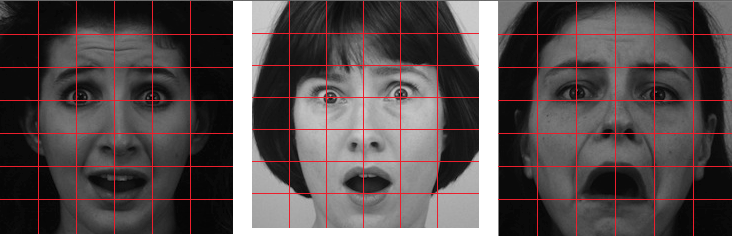
\includegraphics[scale=0.3]{figures/implementation_weight_example} 
\newline
\caption{Example of division into regions of face images from the KDEF database}
\label{implementation_weight_example}
\end{center} 
\end{figure}

\noindent GIVE RESULTS WITH WEIGHTS APPLIED
\newline

\noindent Another way to improve the LBP operator would be to use one with larger scale, hence modify the radius of the circular operator; for example, $ LBP_{12,2.5}^{u^2} $ or $ LBP_{16,4.0}^{u^2} $ (with $ P = 12 $ and $ R = 2.5 $ or with $ P = 16 $ and $ R = 4.0 $). This implies to use the bilinear interpolation because sampling points do not fall exactly on pixels, as seen in Chapter~\ref{chap:lbp}. However, using bilinear interpolation is more computationally expensive. A good compromise has to be found between computation time and accuracy rate.
\newline

\subsection{Combination of feature extraction methods}

\vspace{\baselineskip}
\noindent To improve the accuracy of LBP feature extraction method, another feature extraction method can be used and combined with it. 
\newline

\noindent  For example, a method has been proposed by Liao et al. \cite{LIA09}, where they combine LBP and Gabor filter. It is called Dominant Local Binary Patterns (DLBP), and is robust against change of lighting, image rotation and image noise.  It works by using the most recurrent patterns of the LBP method to obtain more information on the texture. It also uses the Gabor method to add global texture information to one already obtained by LBP. It works based on the circularly symmetric Gabor filter responses \cite{LIA09}. Figure~\ref{combination_lbp_gabor} contains two face images of the YaleB face database , and shows the robustness of the combination against change in lighting. Image (a) is the original image with different lighting conditions, and image (b) is the preprocessed image with the Gabor wavelets. Image (c) is the same image, mapped with the LBP operator. Finally, image (d) is the preprocessed image with the combination of the two methods \cite{GOH11}.
\newline

\begin{figure}[!h]
\begin{center}
\noindent 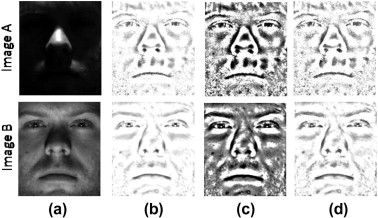
\includegraphics[scale=1]{figures/combination_lbp_gabor} 
\newline

\caption{2 face images of the YaleB face database (a) when processed with Gabor wavelets (b), LBP (c), and Gabor wavelets+LBP (d)\cite{GOH11}}
\label{combination_lbp_gabor}
\end{center} 
\end{figure}

\noindent  LBP has also been combined with the Scale Invariant Feature Transform descriptor (SIFT), which is a ROI descriptor. This descriptor is robust against image rotation, image translations, scaling and lighting variations. Heikkila et al. introduced a combination of the SIFT descriptor with the LBP operator \cite{HEI09}.
\newline

\addtocontents{toc}{\bigskip}
\cleardoublepage
\phantomsection
%\label{bib:mybiblio}
\bibliography{bib/mybib}
\addtocontents{toc}{\bigskip}
\phantomsection
\cleardoublepage
\appendix
\chapter{Appendix A name}\label{ch:appAlabel}
Here is the first appendix

\end{document}
